% CVPR 2026 Paper Template; see https://github.com/cvpr-org/author-kit

\documentclass[10pt,twocolumn,letterpaper]{article}

%%%%%%%%% PAPER TYPE  - PLEASE UPDATE FOR FINAL VERSION
% \usepackage{cvpr}              % To produce the CAMERA-READY version
% \usepackage[review]{cvpr}      % To produce the REVIEW version
\usepackage[pagenumbers]{cvpr} % To force page numbers, e.g. for an arXiv version

% Import additional packages in the preamble file, before hyperref
%% Packages and macros for the LeLunar draft. Loaded before hyperref.

%% Local XeTeX/tectonic builds cannot load the Times (ptm) fonts that cvpr.sty requests;
%% use a Times clone there so page breaks match a pdfLaTeX build. pdfLaTeX is unaffected.
\usepackage{iftex}
\ifXeTeX
  \usepackage{fontspec}
  \setmainfont{texgyretermes}[Extension=.otf, UprightFont=*-regular, BoldFont=*-bold,
    ItalicFont=*-italic, BoldItalicFont=*-bolditalic]
  \setsansfont{texgyreheros}[Extension=.otf, UprightFont=*-regular, BoldFont=*-bold,
    ItalicFont=*-italic, BoldItalicFont=*-bolditalic]
\fi

\usepackage{multirow}
\usepackage{makecell}
\usepackage{tikz}
\usetikzlibrary{arrows.meta,positioning,fit,calc,backgrounds,shapes.geometric}
\usepackage{pifont}

%% Inline annotations; switch off for submission by uncommenting the two lines below.
\newcommand{\red}[1]{{\color{red}#1}}
\newcommand{\todo}[1]{{\color{red}#1}}
\newcommand{\TODO}[1]{\textbf{\color{red}[TODO: #1]}}
% \renewcommand{\TODO}[1]{}
% \renewcommand{\todo}[1]{#1}

\newcommand{\method}{LeLunar\xspace}
\newcommand{\gap}{\ensuremath{\Delta}\xspace}
\newcommand{\share}{\ensuremath{S}\xspace}
\newcommand{\cmark}{\ding{51}}
\newcommand{\xmark}{\ding{55}}
\newcommand{\LN}{\operatorname{LN}}
\newcommand{\sg}{\operatorname{sg}}
\DeclareMathOperator*{\E}{\mathbb{E}}


\definecolor{cvprblue}{rgb}{0.21,0.49,0.74}
\usepackage[pagebackref,breaklinks,colorlinks,allcolors=cvprblue]{hyperref}

%%%%%%%%% PAPER ID  - PLEASE UPDATE
\def\paperID{*****} % *** Enter the Paper ID here
\def\confName{CVPR}
\def\confYear{2027}

\title{\method: From Raw Orbital Products to a Latent World Model of the Lunar Surface}

\author{Sujit Roy\thanks{Equal contribution.}\\
The University of Alabama in Huntsville\\
NASA Marshall Space Flight Center\\
Huntsville, AL, USA\\
{\tt\small sujit.roy@nasa.gov}
\and
Himanshu Patil\footnotemark[1]\\
The University of Alabama in Huntsville\\
Huntsville, AL, USA\\
{\tt\small hap0020@uah.edu}
}

\begin{document}
{\renewcommand*{\thefootnote}{\fnsymbol{footnote}}\maketitle}
\begin{abstract}
Ten instruments on four missions have mapped the Moon, but their products sit in the archive as raw per-image records and global maps with incompatible projections, resolutions and units, and labels are scarce. We present \method, a latent world model of the lunar surface, together with the co-registered corpus we build to train it. From these raw products we build a corpus of 10,629 footprints of 60\,km anchored to the GRAIL gravity grid, with 30 global map layers cut once per footprint at native resolution. Each footprint carries up to 500 Wide Angle Camera observations chosen for illumination diversity, each with its acquisition geometry, and 500\,m sub-tiles with 1\,m Narrow Angle Camera images and 3\,m stereo terrain; splits follow map zones and share no ground. \method treats a footprint as a persistent state seen through instruments. An encoder estimates the state from one or more partially masked observations, and a predictor, told which product to predict and the sun under which it was recorded, predicts the token grid that a moving-average encoder produces for that product. Every product is tokenized at its native resolution, so that a token covers the same ground cell in every product. Training this way has a failure mode the loss hides: a position code, in which tokens encode where they are rather than what the ground looks like, while the loss, within-image rank and VICReg penalties all improve. We explain why these signals are blind, show that two common regularizers push toward the shortcut, and give a cross-sample monitor that flagged every failure we analyzed. Frozen \method features detect craters on par with a masked-token lunar foundation model and gain 0.23 mAP$_{50}$ from a second input product, probes recover relief and albedo from a single image, and predicted shadows follow the sun the predictor is given (AUC 0.89 with the true sun, 0.59 with another).
\end{abstract}

\section{Introduction}
\label{sec:intro}

The Moon is among the best-observed bodies in the solar system. Since 2009 the Lunar Reconnaissance Orbiter (LRO) has returned camera images~\cite{robinson2010lunar}, laser altimetry~\cite{smith2010lunar}, thermal radiometry~\cite{paige2010lunar} and radar~\cite{nozette2010lunar}; Kaguya added multiband imagery and stereo topography~\cite{kato2010kaguya,ohtake2008performance}, GRAIL mapped the gravity field~\cite{zuber2013gravity} and Lunar Prospector the near-surface hydrogen~\cite{binder1998lunar,lawrence2022global}. Yet this archive is not a dataset. Camera images are stored as raw experiment data records, uncalibrated and unprojected, each with its own viewing and illumination geometry. Global maps come at resolutions from 60\,m to 20\,km, in different projections, units and missing-value conventions. Before a model can learn from several instruments at once, their products have to be brought onto the same ground.

Earth observation faced a milder version of this problem and answered it with foundation models pretrained on co-registered multi-sensor archives~\cite{cong2022satmae,fuller2023croma,jakubik2025terramind,tseng2025galileo,astruc2025anysat}. The first lunar foundation models appeared in 2026~\cite{fraccaro2026multimodal,gironamata2026lunarfm,prasad2026moonstone}. All three are trained by reconstructing masked pixels or tokens, resample their inputs to a shared grid, and treat each tile as an independent sample.

We take a different view. The lunar surface is a persistent state: topography, albedo, roughness and composition change on geological time scales. Static maps measure this state directly. A camera image is a rendering of it under a particular sun, and on an airless body the rendering is governed by little other than topography, albedo and illumination. Observations of the same footprint under different suns are therefore views of one state, and a model that must predict one view from another, given the geometry of the target, has to represent the terrain and how light acts on it. This is the structure of a world model~\cite{ha2018recurrent,lecun2022path}: a state estimated from observations and a predictor that rolls the state forward under a control variable. Here the control variable is the acquisition geometry rather than an action, and there is no time axis.

Learning such a model needs data that the archive does not provide: many observations of the same ground under different suns, each with its geometry, co-registered with the static maps at their native resolutions. SomBench~\cite{patil2026sombench} already calibrates the LROC records, orthorectifies them onto the LOLA--Kaguya terrain model and harmonizes the global maps into per-zone projections. It tiles each image on its own windows, however, so a sample holds one view of its ground. On these inputs we build a footprint-anchored corpus (\cref{sec:dataset}). Its 10,629 footprints of 60\,km are anchored to the GRAIL gravity grid. The 30 static layers are cut once per footprint at native resolution and shared by all its observations. Each footprint keeps up to 500 Wide Angle Camera (WAC) observations on identical bounds, selected across bins of incidence and sun azimuth, about 52 per covered footprint on average. It is subdivided into 500\,m sub-tiles that carry 1\,m Narrow Angle Camera (NAC) images and 3\,m stereo terrain models. Splits follow map zones, and a seam rule ensures that no two footprints, and hence no two splits, share ground.

On this corpus we train \method (\cref{sec:method}), a joint-embedding predictive architecture~\cite{assran2023self,bardes2024revisiting}. Each product is tokenized by its own stem at its native resolution, so that a token covers the same ground cell in every product. An encoder reads one or more partially masked observations of a footprint. A predictor, given the target product and its sun, predicts the token grid that an exponential moving average (EMA) of the encoder produces from the actual target observation. A second head predicts a per-cell state that must agree across the observations of the footprint. Nothing is reconstructed in pixel space.

This kind of model can fail in a way that is easy to miss (\cref{sec:collapse}). Much of a target is unpredictable from the source at the token level, while source and target share information about token position and product identity. The model can lower its loss by encoding that shared information instead of the ground. We call the result a position code. It is related to the positional collapse that CAPI reported for latent masked image modeling~\cite{darcet2025cluster}, but here it comes with a falling loss, a rising within-image rank and a shrinking VICReg penalty. We explain why, show that two standard regularizers favor it, and give a cross-sample monitor that costs one cosine per target.

Our contributions are:
\begin{itemize}
  \item a footprint-anchored corpus on the SomBench inputs: GRAIL-grid footprints with static layers cut once at native pixels, up to 500 illumination-diverse WAC observations per footprint on identical bounds with their geometry, 500\,m sub-tiles with NAC, stereo terrain and per-sub-tile static-map means, and zone splits whose seam ownership leaves no shared ground (\cref{sec:dataset});
  \item \method, a latent world model of the surface with ground-cell-aligned native-resolution tokens, a multi-observation evidence encoder, a predictor conditioned on the target product and its illumination, and a state head that ties the observations of a footprint together (\cref{sec:method});
  \item a characterization of position-code collapse in a cross-modal JEPA with continuous targets, an explanation of why the loss, within-tile rank and VICReg penalties cannot see it, and a cross-sample monitor that detected all seven failures we analyzed (\cref{sec:collapse});
  \item experiments on crater detection, shape and albedo from shading and a sun-swap test, which show that frozen features match a masked-token lunar foundation model, gain substantially from a second product, and respond to the sun the predictor is given (\cref{sec:experiments}).
\end{itemize}

\section{Related Work}
\label{sec:related}

\paragraph{Lunar datasets and models.} Machine learning on the Moon has mostly used task-specific data: crater catalogs~\cite{robbins2019new,silburt2019lunar,yang2020lunar,tewari2022automated}, boulder and rockfall maps~\cite{bickel2019automated,bickel2020impacts,aussel2025global}, permanently shadowed regions~\cite{bickel2021peering} and single-image topography~\cite{chen2022cnn,sander2026moon}. Three multimodal pretraining corpora appeared in 2026. LunarFM~\cite{gironamata2026lunarfm} resamples 18 global channels to $0.5^\circ$ chips, Moonstone~\cite{prasad2026moonstone} crops one global map stack at 237\,m, and SomBench~\cite{patil2026sombench} tiles 512-pixel windows inside individual LROC image canvases (51.2\,km on a WAC track, 512\,m on a NAC track) with 30 co-registered layers snapped to the image grid. All three store one view per tile. The NASA-IBM lunar foundation model~\cite{fraccaro2026multimodal} trains TerraMind's masked-token recipe on SomBench with acquisition geometry as input tokens, LunarFM is a MultiMAE and Moonstone a modality-grouped MAE; none predicts latents across products, and none exploits repeat observations of the same ground. Our corpus shares its preprocessed inputs with SomBench but is organized by footprint rather than by image, so that one piece of ground carries all of its camera observations. On Mars, MOMO~\cite{purohit2026momo} merges per-sensor MAEs in weight space and Mars-Bench~\cite{purohit2025marsbench} provides a benchmark.

\paragraph{Multi-sensor models in Earth observation.} Most multi-sensor models resample all inputs to one grid~\cite{fuller2023croma,xiong2024neural,jakubik2025terramind,tseng2025galileo}. Others scale positional encodings by ground distance~\cite{reed2023scale,irvin2023usat,forgaard2026thor} or use a patch size per band or sensor~\cite{irvin2023usat,wang2025towards,labatie2026maestro}. OmniSat and AnySat~\cite{astruc2024omnisat,astruc2025anysat} split all modalities into the same ground cells, as we do, but fuse the modalities of a cell into one token; we keep one token grid per product so that one product can be predicted from another. Galileo~\cite{tseng2025galileo} has the closest objective: its predictor queries carry the target channel group and attend to the other groups, with EMA targets and a contrastive loss, on a common 10\,m grid. AlphaEarth~\cite{brown2025alphaearth} conditions its decoders on measurement metadata such as radar heading, and the NASA-IBM model gives its encoder illumination angles as text tokens; we are not aware of a JEPA whose predictor is conditioned on the illumination of the target. Location encoders on the sphere~\cite{mai2020multi,klemmer2025satclip,russwurm2024geographic} add a geographic prior; we use Slepian functions~\cite{simons2006spatiospectral,rao2026localized} and keep the prior out of the evidence path.

\paragraph{JEPAs and world models.} I-JEPA~\cite{assran2023self} predicts the representations of masked regions from a visible region with targets from an EMA encoder, in the line of BYOL, DINO, iBOT and data2vec~\cite{grill2020bootstrap,caron2021emerging,zhou2022ibot,baevski2022data2vec}. V-JEPA~\cite{bardes2024revisiting,assran2025vjepa} extends this to video, and V-JEPA~2.1~\cite{murlabadia2026vjepa} adds supervision at several depths and a loss on visible tokens, both of which we use. Cross-modal latent prediction exists for audio and video~\cite{haliassos2023jointly} and, with pooled embeddings, for remote sensing~\cite{choudhury2026xjepa,hossain2026crjepa}. World models predict future state representations given actions~\cite{ha2018recurrent,lecun2022path}; recent visual ones freeze a pretrained encoder and train only the predictor~\cite{zhou2024dinowm,bar2025navigation,assran2025vjepa}, so collapse is not their concern. \method trains encoder and predictor jointly from scratch, replaces time and actions by acquisition geometry, and inherits the collapse problems of joint-embedding training.

\paragraph{Collapse and shortcuts.} Joint-embedding methods can collapse to a constant or to a low-dimensional subspace~\cite{jing2022understanding,hua2021feature}. VICReg~\cite{bardes2022vicreg} and Barlow Twins~\cite{zbontar2021barlow} regularize batch statistics, C-JEPA~\cite{mo2024connecting} adds VICReg to I-JEPA, and LeJEPA~\cite{balestriero2025lejepa} pushes embeddings toward an isotropic Gaussian. RankMe~\cite{garrido2023rankme} and LiDAR~\cite{thilak2024lidar} read quality off the embedding spectrum, and Latent MIM~\cite{wei2024towards} tracks the cosine between embeddings of different images. A model can also satisfy its objective without content: context prediction learned patch location from chromatic aberration~\cite{doersch2015unsupervised}, JEPAs can lock onto slow, trivially predictable features~\cite{sobal2022joint}, I-JEPA overfits to location unless mask-token positions are stochastic~\cite{bar2024stochastic}, and CAPI~\cite{darcet2025cluster} saw latent masked image models predict the position of masked tokens instead of their content. Absolute position leaks through zero padding~\cite{islam2020much,kayhan2020translation}, and self-supervised ViTs carry input-independent positional channels~\cite{yang2024denoising,pawlowsky2026dino}. We characterize this shortcut quantitatively in a cross-modal JEPA with continuous targets and show which monitors see it.

\section{From Raw Products to Co-Registered Footprints}
\label{sec:dataset}

\begin{figure*}[t]
  \centering
  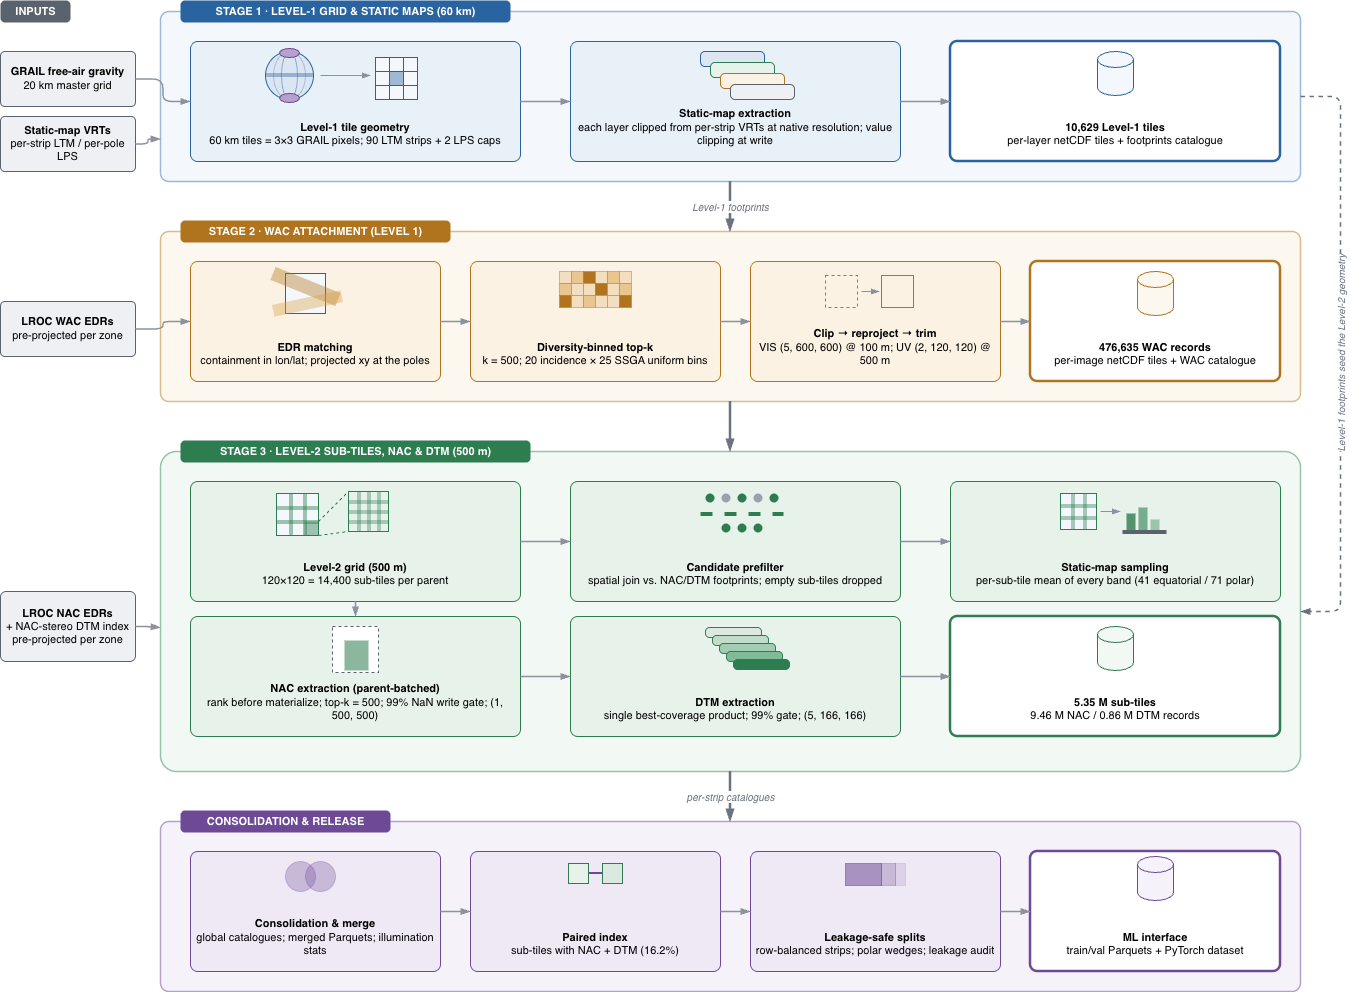
\includegraphics[width=\textwidth]{figures/footprint_anchored.png}
  \caption{Corpus construction. Stage~1 lays 60\,km footprints ($3\times3$ GRAIL pixels) over 90 LTM strips and two polar caps and clips every static layer at native resolution. Stage~2 keeps up to 500 illumination-diverse WAC observations per footprint. Stage~3 cuts each footprint into 500\,m sub-tiles that carry per-sub-tile static means, NAC images and the best stereo terrain model. Consolidation builds the merged and paired catalogs and the splits. Heavy borders mark stored artifacts.}
  \label{fig:pipeline}
\end{figure*}

SomBench~\cite{patil2026sombench} cuts its tiles inside individual image canvases, one view per tile, which suits benchmarks posed on one image. A world model needs the reverse: the ground is the sample and the images are views of it, aligned pixel for pixel under many suns. We reuse SomBench's raw image selection and preprocessing and build a different corpus on top (\cref{fig:pipeline,tab:contrast}). The supplement (\cref{sec:supp_data}) gives the long form of every stage and lists all 34 layers.

\begin{table}[t]
  \centering
  \footnotesize
  \setlength{\tabcolsep}{3pt}
  \caption{Two corpora built from the same raw products.}
  \label{tab:contrast}
  \begin{tabular}{@{}p{0.22\linewidth}p{0.36\linewidth}p{0.38\linewidth}@{}}
    \toprule
    & Image-anchored (SomBench) & Footprint-anchored (ours) \\
    \midrule
    Sample unit       & 512\,px window in one record      & 60\,km footprint, $3\times3$ GRAIL px \\
    Images per place  & one per tile                      & up to 500 on identical bounds \\
    Static layers     & re-clipped per record (42.5\,TB)  & once per footprint (9.5\,TB) \\
    NAC--WAC link     & independent tracks                & sub-tiles keyed to their parent \\
    Ground overlap    & windows may overlap               & none (seam ownership) \\
    Geometry          & one set per tile                  & per observation, plus series statistics \\
    \bottomrule
  \end{tabular}
\end{table}

\subsection{Source products and preprocessing}
\label{sec:sources}

Camera observations are experiment data records (EDRs) of the LRO Wide and Narrow Angle Cameras~\cite{robinson2010lunar}, drawn from the SomBench pools of 63,468 WAC and 11,302 NAC records, plus 585 NAC stereo terrain models (DTMs) at 2--5\,m~\cite{henriksen2017extracting}. Static layers come from ten instruments on four missions: SLDEM2015 topography~\cite{barker2016new}, LOLA roughness~\cite{kreslavsky2013lunar,neumann2015copernican}, WAC mosaics and TiO$_2$~\cite{speyerer2011lunar,boyd2012lunar,wagner2015new,sato2017lunar}, Kaguya MI reflectance, mineralogy and space weathering~\cite{ohtake2008performance,lemelin2016global,trang2019improved}, Diviner rock abundance, regolith temperature, H-parameter and bolometric temperature~\cite{paige2010lunar,powell2023high,hayne2017global,williams2017global}, Mini-RF radar~\cite{nozette2010lunar,fassett2024improved}, the USGS geologic map~\cite{fortezzo2020release} and GRAIL gravity~\cite{zuber2013gravity}. Fourteen more layers serve the polar caps~\cite{williams2019seasonal,schorghofer2020mapping,mazarico2011illumination,lemelin2016improved,lemelin2022compositional,lawrence2022global}.

\paragraph{Preprocessing.}
\label{sec:preprocessing}
As in SomBench, EDRs are calibrated~\cite{mahanti2016inflight,humm2016flight} and echo-corrected with USGS ISIS\footnote{\url{https://doi.org/10.5066/P13YBMZA}} and orthorectified onto SLDEM2015 with the Ames Stereo Pipeline~\cite{beyer2018ames}. Each image is projected into the Lunar Transverse Mercator (LTM) zone~\cite{mcclernan2025lunar} holding most of its area. Static maps are harmonized to equidistant cylindrical and exposed as one virtual raster (VRT) per LTM strip and per Lunar Polar Stereographic (LPS) cap.

\subsection{Footprints on the GRAIL grid}
\label{sec:grid}

GRAIL gravity at 20\,km is global and independent of illumination, so it is the master grid. A Level-1 footprint is a $3\times3$ block of GRAIL pixels, 60\,km on a side in its region's projection and aligned to GRAIL pixel edges, so the master grid is never resampled. The regions are 90 LTM strips of $8^\circ$ longitude, 45 per hemisphere up to $|\phi|{=}82^\circ$, and two LPS caps; zones 1 and 45 are inset $0.5^\circ$ from the antimeridian. Footprints are laid without overlap, which would only duplicate: static pixels on shared ground are identical, and a WAC record clipped twice keeps its geometry.

\paragraph{Seam ownership.} A footprint belongs to the region holding its center. Each region tiles its own projected raster, so edge footprints of neighboring regions could cover up to 94\% of the same ground. Of two overlapping candidates from different regions we create only the one with more of its area inside its own region, with ties to a fixed region ranking. Each strip job derives its neighbors' candidates from their GRAIL rasters, so the 92 jobs stay independent. Over the $0$--$82^\circ$ band, the center rule covers 94\% of the ground with 5.9\% twice; ownership covers 82\% with none twice. \TODO{refresh counts after the seam repair; \cref{tab:corpus} predates it}

\subsection{Static layers once per footprint}
\label{sec:attach}

A layer of native resolution $r$ is read from the strip's VRT, already in the footprint's projection, and clipped at native pixels to a side of $t = \lfloor 60\,\text{km}/r \rfloor$, from 1000 for SLDEM2015 to 3 for GRAIL. Nothing is reprojected; only GRAIL and Diviner bolometric temperature are resampled within the same projection to restore the $t\times t$ shape. Each layer is extracted once per footprint and shared by all its observations and sub-tiles. SomBench re-clips every layer for every image tile and stores 21.5\,M files in 42.5\,TB; this corpus takes 9.5\,TB.

At write time, categorical bands are snapped to their classes, circular bands wrapped, and every band clipped to its physical range, with NaN kept as a gap. A scan of all sources showed that cubic resampling in the VRTs smeared no-data sentinels into neighbors (FeO up to 2,810\,wt\%, aspect up to $450^\circ$), and found eleven defective NAC products, which are excluded (\cref{sec:supp_data}).

\subsection{Repeat observations with their geometry}
\label{sec:wac}

\begin{figure}[t]
  \centering
  \begin{subfigure}[t]{0.49\linewidth}
    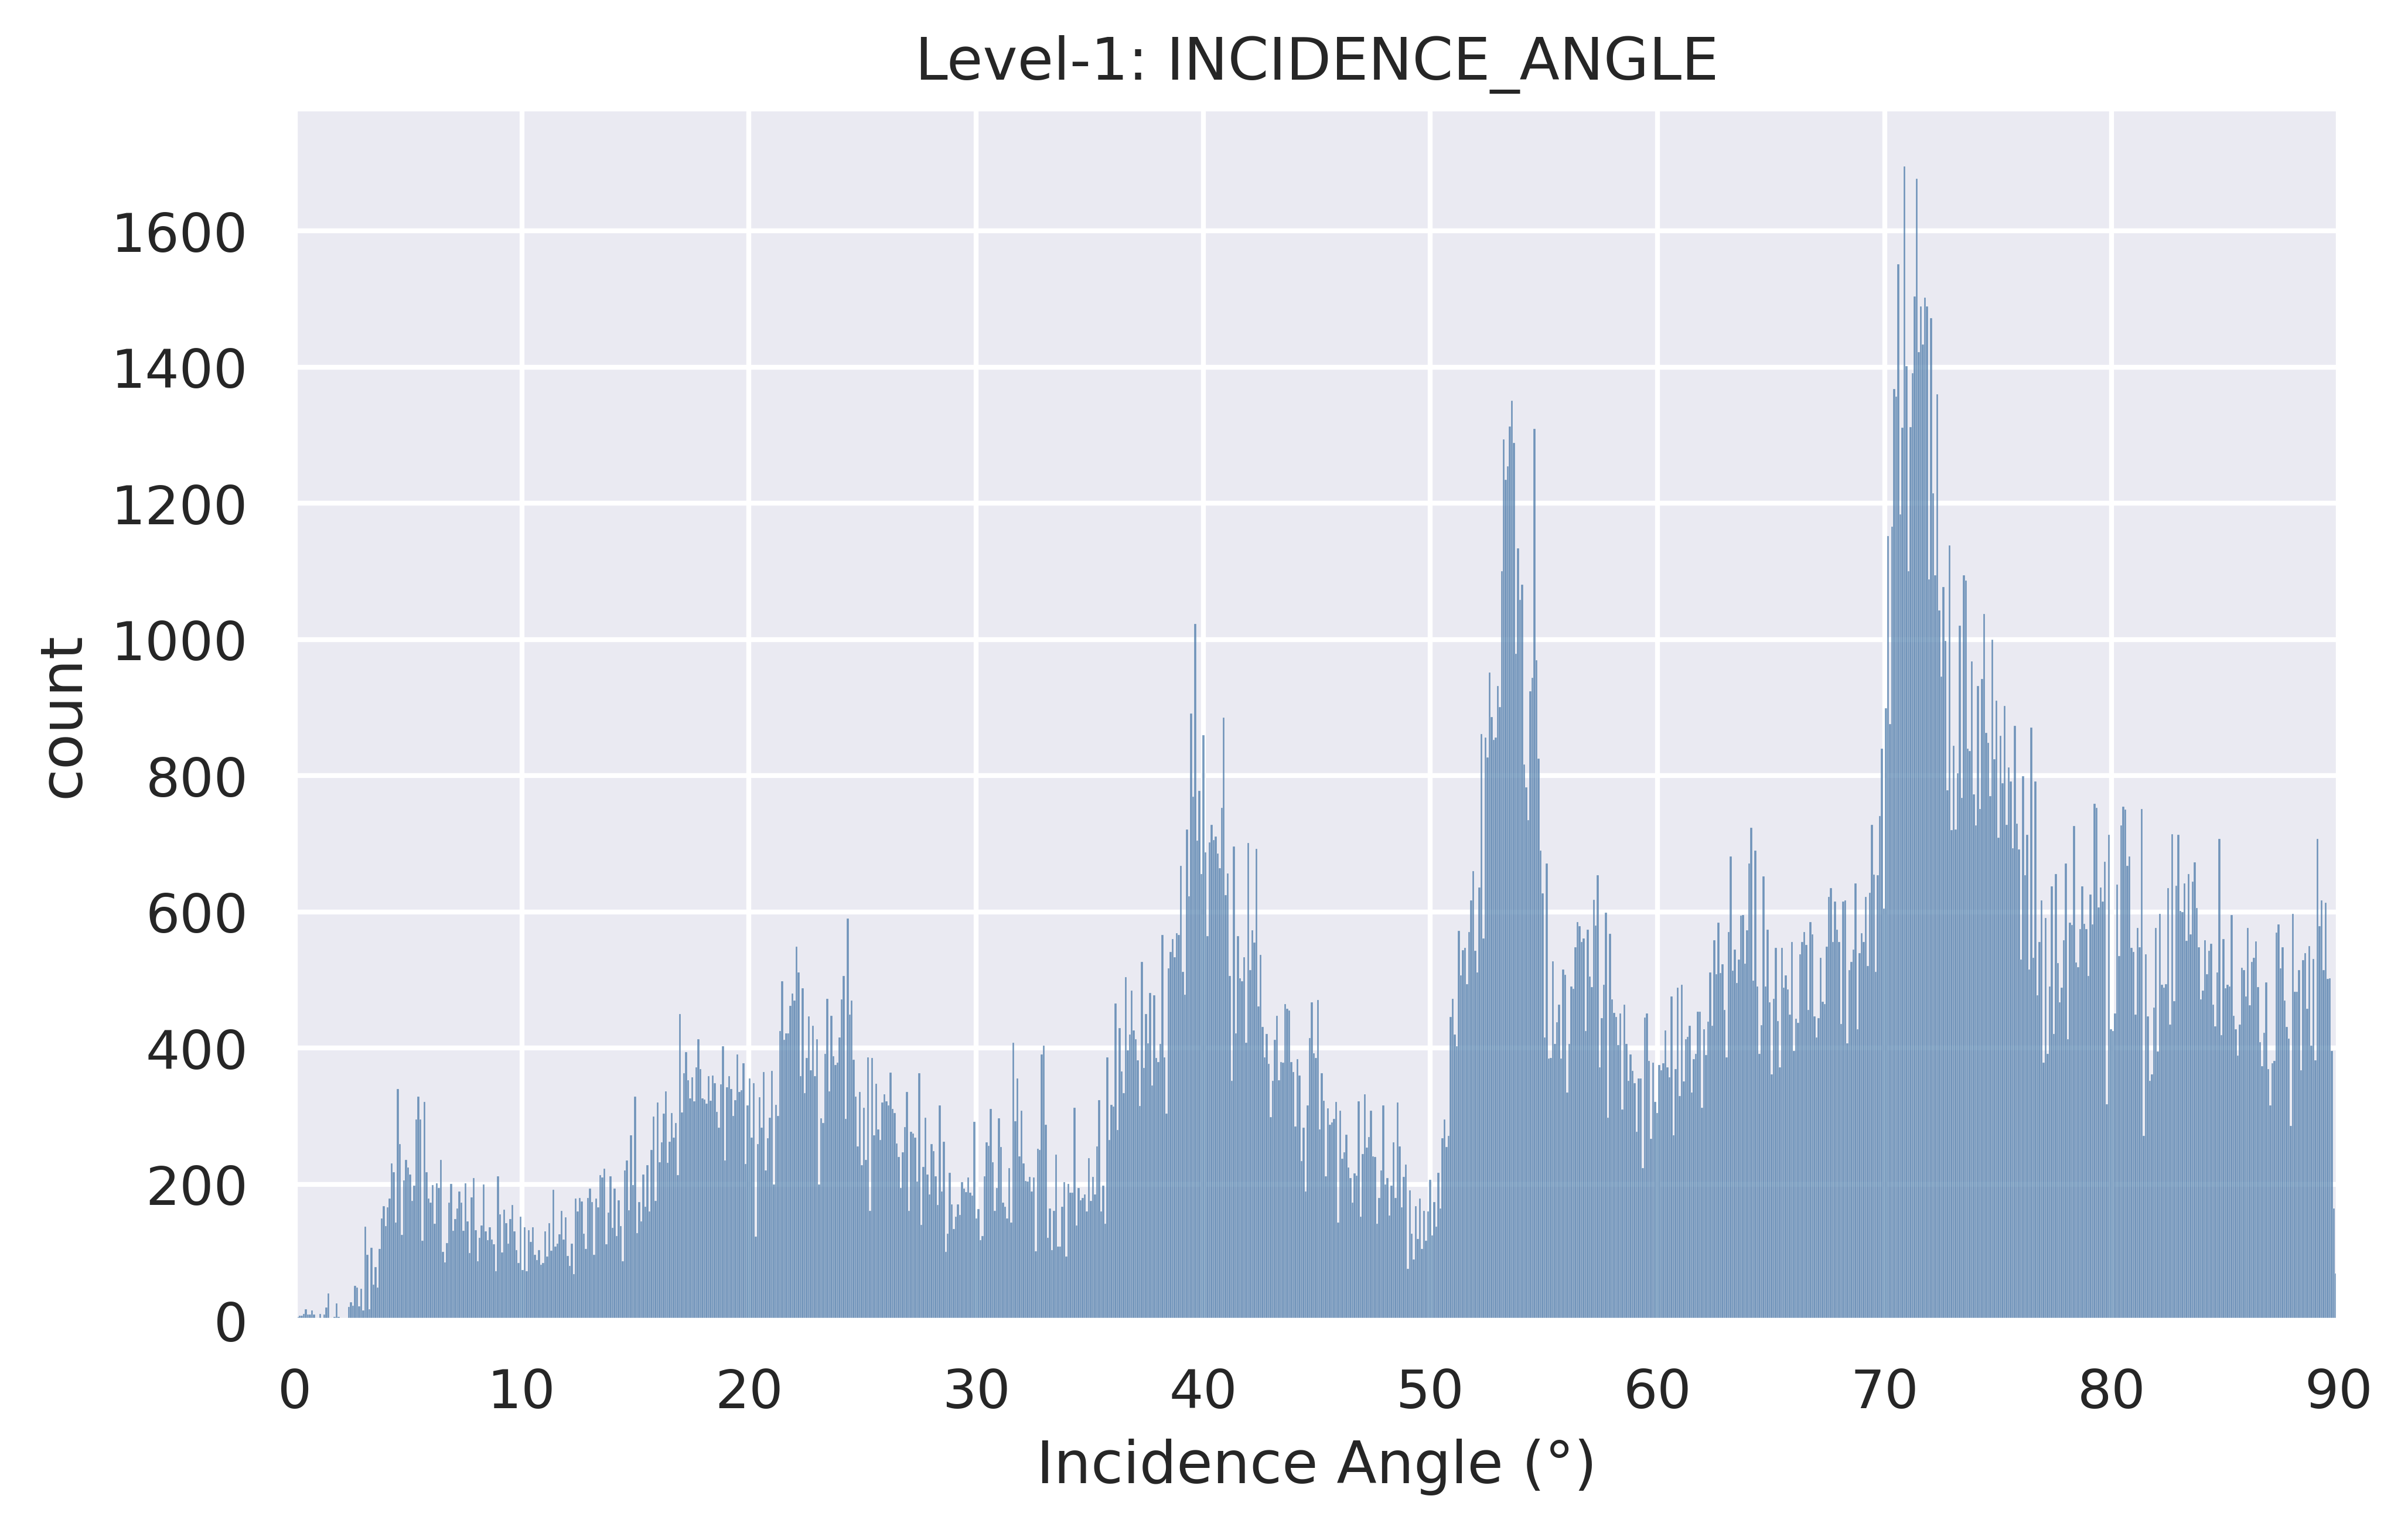
\includegraphics[width=\linewidth]{figures/level1_INCIDENCE_ANGLE.png}
    \caption{Incidence angle.}
  \end{subfigure}\hfill
  \begin{subfigure}[t]{0.49\linewidth}
    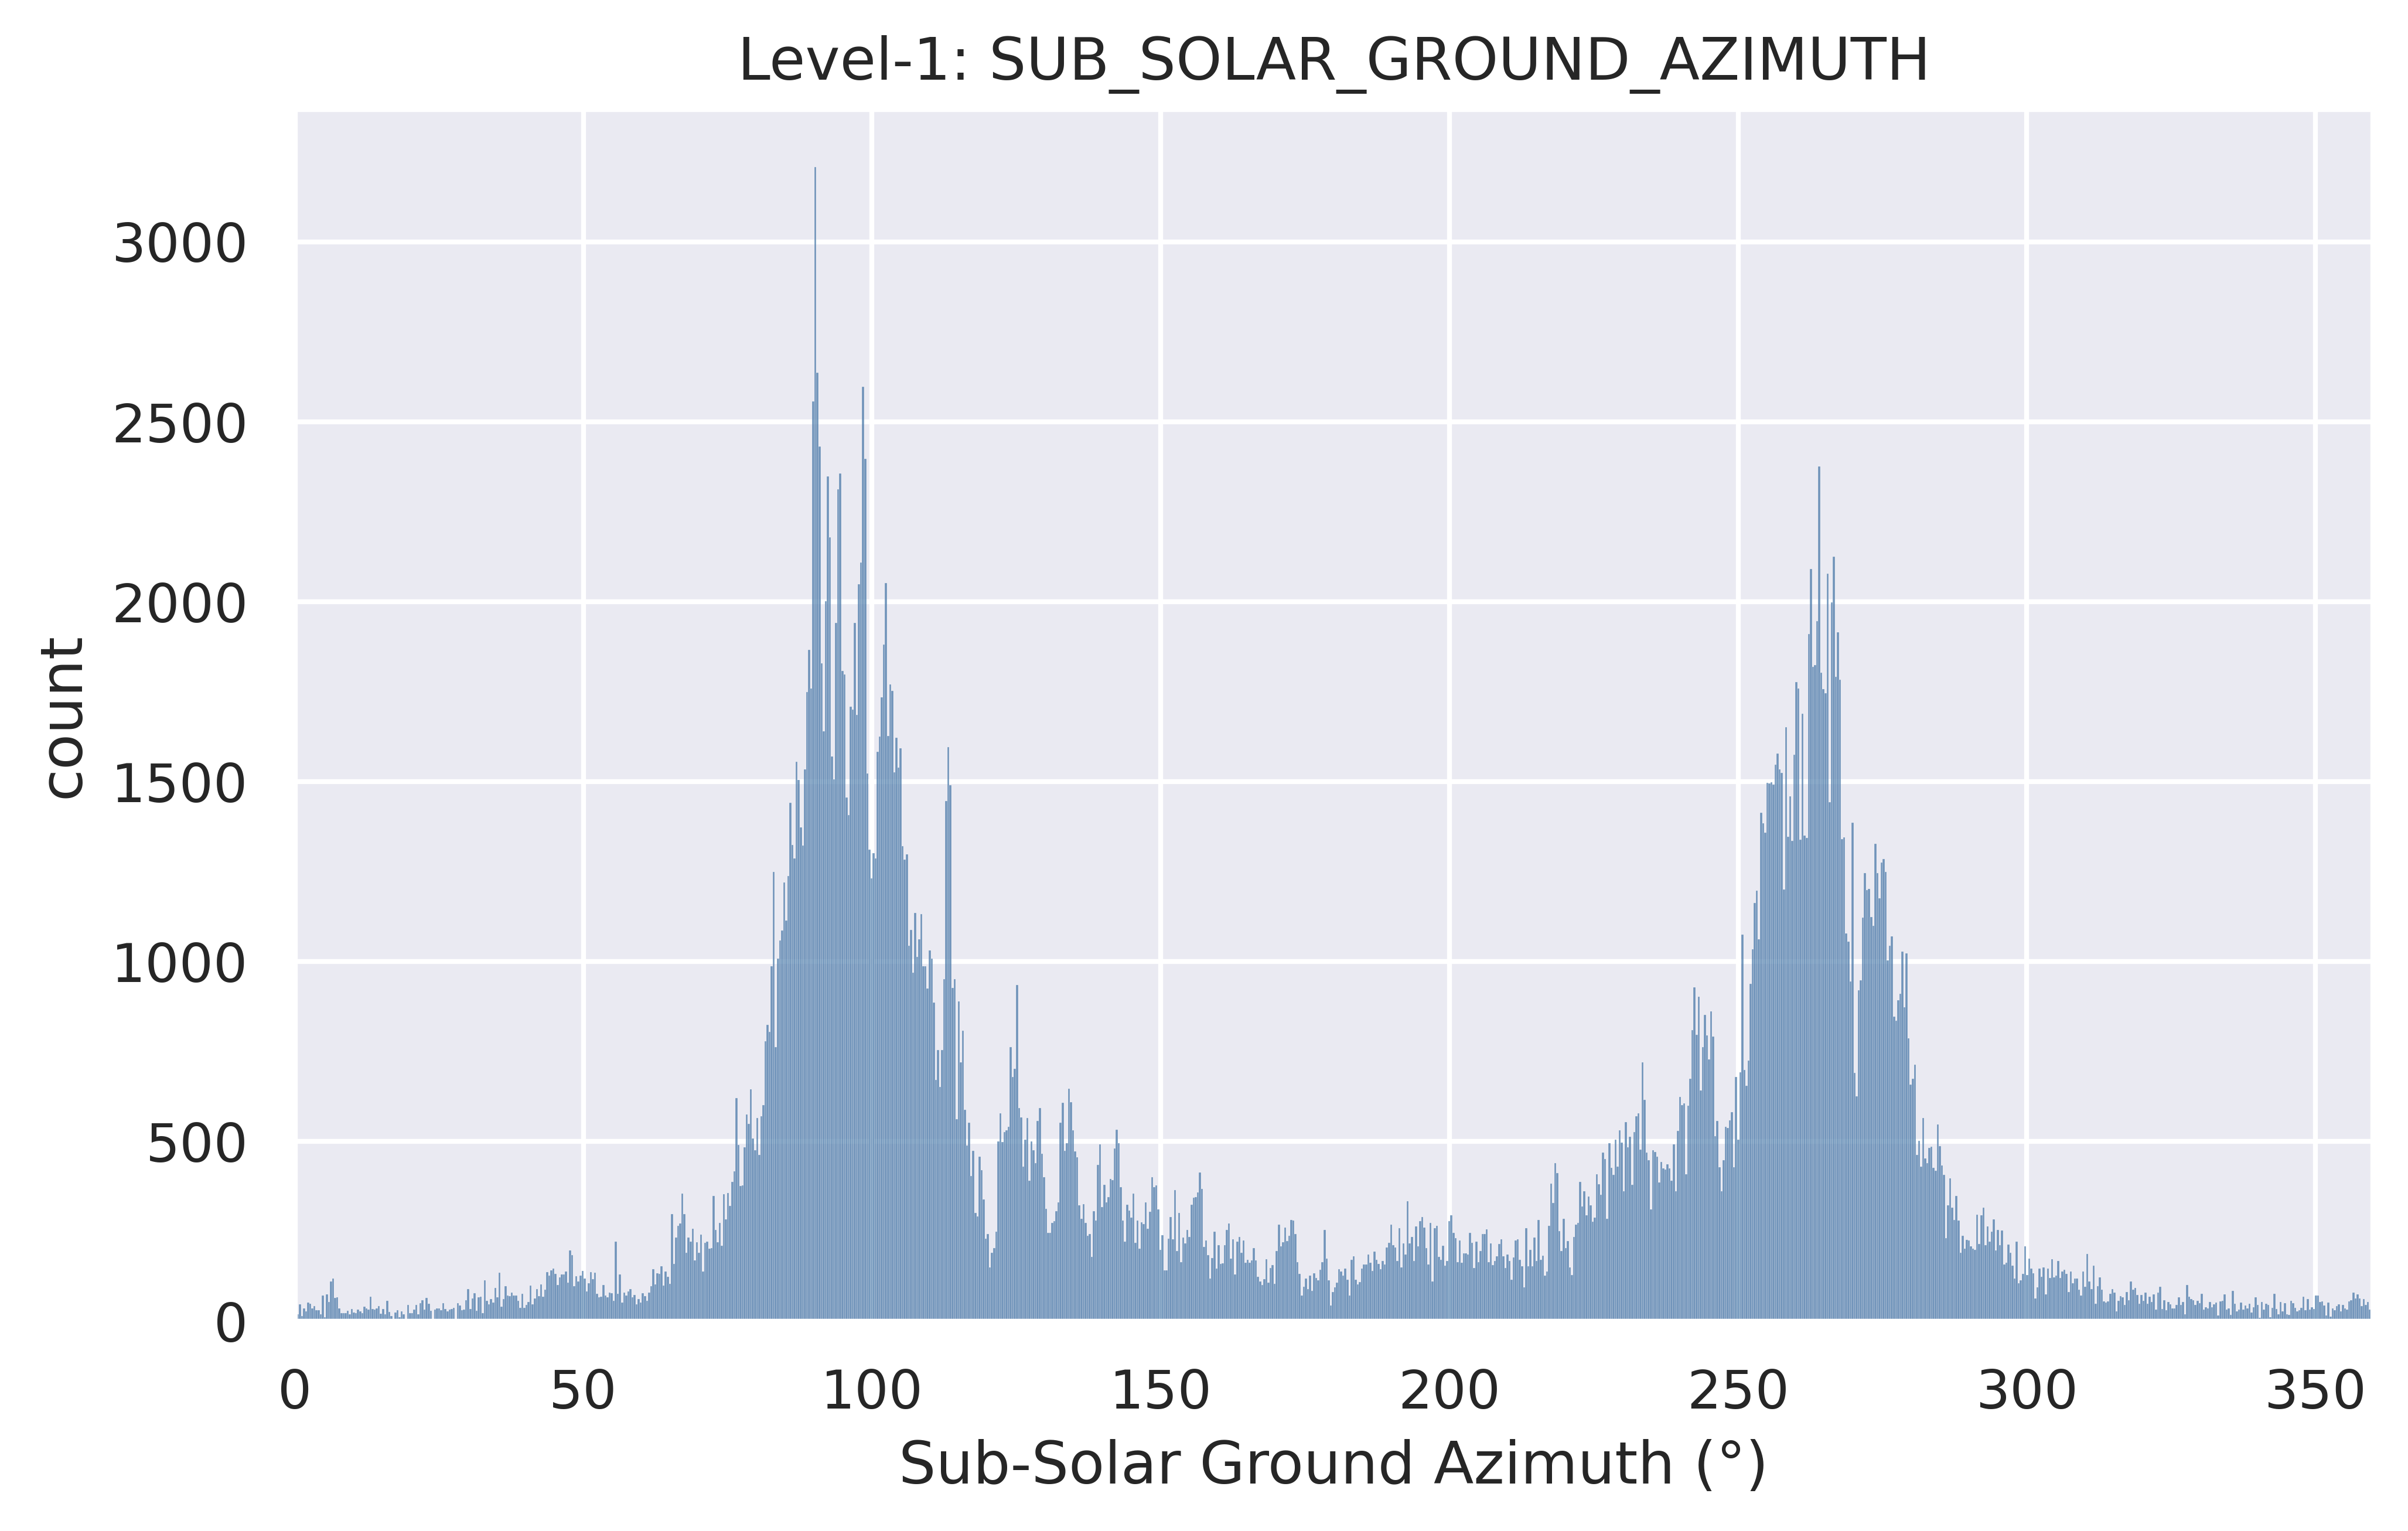
\includegraphics[width=\linewidth]{figures/level1_SUB_SOLAR_GROUND_AZIMUTH.png}
    \caption{Sub-solar ground azimuth.}
  \end{subfigure}
  \caption{Illumination of the 476,635 retained WAC observations. Incidence covers nearly the full $0$--$90^\circ$ range. Azimuth has two modes near $90^\circ$ and $265^\circ$, with smaller counts elsewhere.}
  \label{fig:illum}
\end{figure}

A WAC record is a candidate when its footprint polygon contains the footprint, tested in geographic coordinates, or in LPS coordinates in the caps, where a 60\,km square unprojects to a box hundreds of degrees wide. A record in the footprint's zone is sliced directly. Otherwise the four tile corners are transformed into the record's projection and enveloped, the record is clipped there with a 2-pixel buffer, and only the clip is reprojected and trimmed; incompatible pairs, such as a polar stereographic record and an LTM tile, are rejected.

Up to $k{=}500$ candidates are kept per footprint. They are binned by incidence (20 bins) and sub-solar azimuth ($\operatorname{round}(k/20){=}25$ bins), with edges from each strip's observed range, and drawn round-robin across occupied cells in random order, with five attempts per slot. A record with any missing visible or ultraviolet pixel is rejected. The final pass takes the lowest-NaN candidate of each cell first, so the set spans the sun instead of collapsing onto the cleanest, often near-duplicate, records. An observation is a visible $(5, 600, 600)$ tile at 100\,m and an ultraviolet $(2, 120, 120)$ tile at 500\,m, with incidence, emission, phase, sub-solar azimuth, sub-solar and sub-spacecraft coordinates and north azimuth. The corpus holds 476,635 WAC observations; 86.9\% of footprints have at least one, and a covered footprint has about 52 (\cref{fig:illum}).

\subsection{Sub-tiles with NAC and stereo terrain}
\label{sec:level2}

On a 60\,km footprint, NAC at 1\,m would need 60,000 pixels per side and a swath covers only part of it. Each parent is therefore cut into $120\times120$ sub-tiles of 500\,m with a parent key. A spatial join drops sub-tiles with no NAC or DTM candidate before any raster is read, and an averaging read of the parent gives every static band as a per-sub-tile mean (41 bands equatorial, 71 polar).

NAC observations are chosen by the same sampler and placed at their true position in a $(1, 500, 500)$ canvas, so partial coverage stays NaN; canvases above 99\% NaN are not written. Each product is opened once per parent, and a first pass counts valid pixels per sub-tile without building canvases. Only the selected pairs are then materialized, avoiding about $5\times10^8$ naive clip-and-reproject operations. Each sub-tile also gets the DTM with the lowest elevation NaN: elevation, slope, aspect and its sine and cosine at $(5, 166, 166)$. Of the 5,354,773 retained sub-tiles, 86.6\% have NAC and 16.0\% a DTM.

\subsection{Records and splits}
\label{sec:splits}

\begin{table}[t]
  \centering
  \footnotesize
  \setlength{\tabcolsep}{4pt}
  \caption{Configuration and scale. Coverage is the share of footprints (WAC) or sub-tiles (NAC, DTM) with at least one record. Counts predate the seam repair of \cref{sec:grid}; the paired count also predates the NAC exclusion.}
  \label{tab:corpus}
  \begin{tabular}{@{}lr@{}}
    \toprule
    Regions                    & 90 LTM strips + 2 LPS caps \\
    Master grid                & GRAIL, 20\,km \\
    Footprint (Level 1)        & 60\,km, $3\times3$ GRAIL px \\
    Sub-tile (Level 2)         & 500\,m, $120\times120$ per parent \\
    WAC per footprint          & $k{=}500$, diversity-binned \\
    NAC per sub-tile           & $k{=}500$, diversity-binned \\
    DTM per sub-tile           & 1, lowest elevation NaN \\
    NaN gate                   & WAC 0\%; NAC, DTM 99\% \\
    \midrule
    Footprints                 & 10,629 \\
    Sub-tiles with NAC or DTM  & 5,354,773 \\
    WAC observations           & 476,635 (86.9\%, $\approx$52 each) \\
    NAC observations           & 9,453,706 (86.6\%) \\
    DTM tiles                  & 856,535 (16.0\%) \\
    Paired NAC + DTM rows      & 1,653,060 \\
    Source WAC / NAC products  & 59,503 / 10,484 \\
    Compressed size            & 9.5\,TB \\
    \bottomrule
  \end{tabular}
\end{table}

Per-strip Parquet catalogs are unioned into a Level-1 index (one row per footprint and WAC observation), a Level-2 index (one row per sub-tile and NAC observation, with the sub-tile's observation count and incidence and azimuth ranges) and a paired NAC and DTM index. Each layer of each tile is a compressed netCDF file with named bands, coordinates and projection.

Splits assign whole LTM strips to train, validation or test, accumulated greedily by row count so that dense strips do not skew the fractions; sub-tiles inherit their parent's split. Each cap is cut into eight longitude wedges, with parents beyond $88^\circ$ pinned to train. The splitter audits records that straddle a strip boundary and refuses splits whose footprints share ground. Pretraining in this paper uses the non-polar Level-1 rows (\cref{tab:corpus}). \TODO{non-polar train and validation footprint counts}

\section{\method: A Latent World Model of the Surface}
\label{sec:method}

\begin{figure*}[t]
  \centering
  \resizebox{\textwidth}{!}{% Overview figure: (a) per-product stems map every raster to the same token grid,
% (b) the world model: observations -> encoder -> evidence; predictor told the target
% product and its geometry; state head tied to the EMA projection of the targets.
\begin{tikzpicture}[
    font=\footnotesize,
    >={Stealth[length=1.6mm]},
    box/.style={draw, rounded corners=2pt, align=center, inner sep=3pt, minimum height=0.9cm},
    enc/.style={box, fill=blue!8, minimum width=1.9cm},
    pred/.style={box, fill=orange!12, minimum width=2.2cm},
    ema/.style={box, fill=gray!10, minimum width=1.9cm, dashed},
    lab/.style={font=\scriptsize, align=center},
    plab/.style={font=\scriptsize, fill=white, inner sep=1pt},
  ]

  % Token grid: \tgrid{x}{y}{cells-1}{size}{fill}{masked border?}
  \newcommand{\tgrid}[6]{%
    \foreach \i in {0,...,#3} {\foreach \j in {0,...,#3} {%
      \pgfmathsetmacro{\m}{#6 && (\i<1 || \j>#3-1)}%
      \ifdim\m pt>0.5pt
        \fill[gray!45] ({#1+\i*#4},{#2+\j*#4}) rectangle ++(#4,#4);
      \else
        \fill[#5] ({#1+\i*#4},{#2+\j*#4}) rectangle ++(#4,#4);
      \fi
      \draw[white, line width=0.25pt] ({#1+\i*#4},{#2+\j*#4}) rectangle ++(#4,#4);
    }}}
  % Raster with n x n pixels: \raster{x}{y}{n}{side}{color}
  \newcommand{\raster}[5]{%
    \pgfmathsetmacro{\px}{#4/#3}
    \foreach \i in {1,...,#3} {\foreach \j in {1,...,#3} {%
      \pgfmathsetmacro{\v}{int(50+25*sin(\i*47+\j*29)*cos(\i*13-\j*31)+15*sin(\j*71))}%
      \fill[#5!\v!white] ({#1+(\i-1)*\px},{#2+(\j-1)*\px}) rectangle ++(\px,\px);
    }}
    \draw[black!60] (#1,#2) rectangle ++(#4,#4);}

  % ---------------- (a) one token, one ground cell ----------------
  \node[lab, anchor=west] at (-0.2,3.9) {\textbf{(a)} one token, one ground cell};
  \raster{0}{2.1}{16}{1.05}{brown}
  \raster{0}{0.85}{10}{1.05}{blue}
  \raster{0}{-0.4}{4}{1.05}{teal}
  \node[lab, anchor=west] at (1.1,2.62) {DTM\\60\,m, 1000\,px};
  \node[lab, anchor=west] at (1.1,1.37) {WAC\\100\,m, 600\,px};
  \node[lab, anchor=west] at (1.1,0.12) {roughness\\1\,km, 60\,px};
  \draw[->] (2.75,2.62) -- node[plab, pos=0.5] {$p{=}16$} (4.0,1.62);
  \draw[->] (2.75,1.37) -- node[plab, pos=0.5] {$p{=}9$} (4.0,1.3);
  \draw[->] (2.75,0.12) -- node[plab, pos=0.5] {$p{=}4$} (4.0,0.98);
  \tgrid{4.1}{0.7}{7}{0.15}{blue!30}{0}
  \node[lab] at (4.7,0.3) {$G{\times}G$ tokens,\\$E/G$ per cell};

  % ---------------- (b) world model ----------------
  \begin{scope}[xshift=0.7cm]
  \node[lab, anchor=west] at (5.2,3.9) {\textbf{(b)} estimate the state from observations, predict another product under its sun};

  % source branch (K observations)
  \raster{5.45}{2.05}{16}{0.95}{brown}
  \raster{5.3}{1.9}{10}{0.95}{teal}
  \node[lab] at (5.82,1.62) {observations $X_{1..K}$};
  \draw[->] (6.45,2.42) -- node[above, lab] {$\phi_m$} (6.95,2.42);
  \tgrid{7.0}{1.85}{7}{0.145}{brown!35}{1}
  \node[lab] at (7.58,1.55) {masked};
  \node[lab] at (7.58,3.2) {$+\,\mu_m+\eta(g_m)$};
  \draw[->] (8.25,2.42) -- (8.65,2.42);
  \node[enc] (enc) at (9.6,2.42) {encoder $f_\theta$\\ViT-B, MoE};
  \draw[->] (enc.east) -- node[above, lab] {evidence $z$} (11.35,2.42);

  % state head
  \node[box, fill=green!10, minimum height=0.55cm, font=\scriptsize] (wh) at (10.75,1.3) {state head $\to \hat w$};
  \draw[->] (10.75,2.42) -- (wh.north);
  \node[lab, text=gray, anchor=north] at (10.75,0.98) {$\mathcal{L}_{\text{state}}$};

  % predictor
  \node[pred] (pr) at (12.5,2.42) {predictor $g_\psi$\\cross + self attn.};
  \node[lab] (q) at (12.5,3.45) {queries: $q + \mu_t$ at every cell};
  \draw[->] (q) -- (pr.north);
  \node[box, fill=yellow!20, minimum height=0.6cm] (sun) at (12.5,0.75) {geometry $g_t$ $\to c_t$};
  \draw[->] (sun) -- node[right, lab, pos=0.45] {AdaLN\\+ kv token} (pr.south);
  \draw[->] (pr.east) -- (13.9,2.42);
  \tgrid{14.0}{1.85}{7}{0.145}{orange!45}{0}
  \node[lab] at (14.58,3.2) {$\hat z^{\,l}_t$};

  % target branch
  \raster{5.3}{-0.35}{10}{1.05}{blue}
  \node[lab] at (5.82,-0.62) {target $X_t$ (WAC, sun $g_t$)};
  \draw[->] (6.45,0.17) -- node[above, lab] {$\bar\phi_t$} (6.95,0.17);
  \tgrid{7.0}{-0.4}{7}{0.145}{blue!30}{0}
  \draw[->] (8.25,0.17) -- (8.65,0.17);
  \node[ema] (tenc) at (9.6,0.17) {EMA encoder\\$f_{\bar\theta}$ (full grid)};
  \draw[->] (tenc.east) -- (10.3,0.17) |- (11.2,-0.15) -- (13.9,-0.15);
  \tgrid{14.0}{-0.7}{7}{0.145}{blue!30}{0}
  \node[lab] at (14.58,-1.0) {$\LN(\bar z^{\,l}_t)$};
  \draw[<->, thick, red!70!black] (15.3,2.42) to[bend left=35] node[right, lab, text=red!70!black] {$\mathcal{L}_{\text{obs}}$\\4 depths} (15.3,-0.15);
  \draw[->, dashed, gray] (enc.south) ++(-0.6,0) -- node[left, lab, text=gray] {EMA} ++(0,-1.25);
  \end{scope}
\end{tikzpicture}
}
  \caption{\method. (a) Each product is tokenized by its own stem at its native pixels per token, so that every token covers the same ground cell. (b) The encoder reads one or more partially masked observations of a footprint. The predictor, given the target product and the geometry $g_t$ under which it was recorded, predicts the token grid that the EMA encoder produces from the actual target. A state head predicts a per-cell state that must agree with the EMA projection of the targets.}
  \label{fig:overview}
\end{figure*}

\subsection{Formulation}
\label{sec:formulation}

Let $x$ be a footprint with surface state $s(x)$. The corpus observes $s$ in two ways. Static products $X_m$ measure one aspect of the state directly. Camera images $X_{m,g}$ depend on the state and on the acquisition geometry $g$, six angles that fix the sun and the viewing direction. \method has an encoder $f_\theta$ that estimates a token-grid representation of the state from a set of $K$ partially observed products $\{(X_{m_k}, g_k)\}_{k=1}^{K}$ of the same footprint, and a predictor $g_\psi$ that, given the identity of a target product $t$ and its geometry $g_t$, predicts how $t$ looks in representation space. The representation it must match is produced by an EMA copy of the encoder from the actual target product, which the student never sees. Geometry plays the part that actions play in a world model~\cite{lecun2022path}: the same state rolled out under a different sun must give a different image. Static targets are predicted with a null geometry. A task sampler (\cref{sec:tasks}) fixes $K \in \{1,2,3\}$ sources and $M{=}2$ targets per row. Since each footprint has many camera observations, the same terrain is routinely asked for under suns it was never shown with.

\begin{table}[t]
  \centering
  \footnotesize
  \setlength{\tabcolsep}{2.1pt}
  \caption{Products used for pretraining. $r$: native ground sample distance. $C$: bands. $p$: native pixels per token at $G{=}64$ and $S_{\max}{=}1000$, before and after a kernel floor of 4 (\cref{sec:tokens}). $^\star$Appearance depends on the sun; each observation carries its geometry. The lower block joins in the 12-product runs.}
  \label{tab:modalities}
  \begin{tabular}{@{}llrcc@{}}
    \toprule
    Product & Source & $r$ (m) & $C$ & $p$ \\
    \midrule
    WAC visible$^\star$       & LROC WAC~\cite{robinson2010lunar}      & 100  & 5    & 9 \\
    WAC ultraviolet$^\star$   & LROC WAC                               & 500  & 2    & 2 $\to$ 4 \\
    Elevation                 & SLDEM2015~\cite{barker2016new}         & 60   & 1    & 16 \\
    Slope; aspect             & from elevation                         & 60   & 1; 2 & 16 \\
    643\,nm mosaic            & WAC normalized~\cite{boyd2012lunar}    & 100  & 1    & 9 \\
    Roughness                 & LOLA~\cite{kreslavsky2013lunar}        & 1000 & 1    & 1 $\to$ 4 \\
    \midrule
    Morphologic mosaic        & WAC~\cite{speyerer2011lunar}           & 100  & 1    & 9 \\
    Normalized reflectance    & WAC normalized~\cite{boyd2012lunar}    & 500  & 7    & 2 $\to$ 4 \\
    MI reflectance            & Kaguya MI~\cite{lemelin2016global}     & 60   & 8    & 16 \\
    MI mineralogy             & Kaguya MI~\cite{lemelin2016global}     & 60   & 7    & 16 \\
    TiO$_2$                   & WAC~\cite{sato2017lunar}               & 400  & 1    & 2 $\to$ 4 \\
    \bottomrule
  \end{tabular}
\end{table}

\subsection{One token, one ground cell}
\label{sec:tokens}

A common approach resamples all products to a shared canvas and cuts it into patches. At a $64\times64$ token grid with $4\times4$ patches, this shrinks the 1000\,px topography raster four times and the 600\,px WAC image 2.3 times, and blows the 60\,px roughness map up four times. We instead align tokens to ground cells, as OmniSat and AnySat do~\cite{astruc2024omnisat,astruc2025anysat}, and give every product $m$ its own stem $\phi_m$ whose kernel and stride equal its native pixels per token,
\begin{equation}
  p_m = \max\!\big(k_{\min},\ \operatorname{round}(\min(E/r_m, S_{\max})/G)\big),
  \label{eq:ppt}
\end{equation}
where $E{=}60$\,km is the footprint extent, $r_m$ the ground sample distance and $G$ the grid size. Sub-tile rows (NAC, stereo terrain) use $E{=}500$\,m in the same rule, which gives the 500\,px NAC and 166\,px terrain rasters. The raster is resized to $Gp_m$ pixels per side, which changes it by a few percent unless the floor applies, and $\phi_m$ maps it to a $G\times G$ grid of $D$-dimensional tokens. Every token is then one ground cell of $E/G$ meters (940\,m at $G{=}64$), whatever the product (\cref{tab:modalities}).

\paragraph{Kernel floor.} At $G{=}64$, \cref{eq:ppt} with $k_{\min}{=}1$ gives LOLA roughness one pixel per token. Each token is then a scalar times a fixed vector, so all roughness tokens lie on a line in $\mathbb{R}^D$ (measured effective rank 1), a target that is easy to fit and carries little. A floor $k_{\min}{=}4$ pre-upsamples coarse products so that each token sees a $4\times4$ patch.

\paragraph{Convolutional stems.} A linear patch projection~\cite{dosovitskiy2021image} has to preserve edges and texture through one matrix, so our stems are factorized convolutions~\cite{xiao2021early}: $p_m$ is split into stride-3 and stride-2 stages ($9{=}3{\cdot}3$, $16{=}2^4$, $4{=}2^2$), each a convolution with GroupNorm and GELU, followed by a $1\times1$ projection to $D$. The usual $3\times3$ kernel with padding 1 has a quiet flaw here, a case of the receptive-field offsets that stride and padding produce~\cite{araujo2019computing,alsallakh2021mind}. It centers output $o$ of a stride-$s$ stage on input pixel $so$ rather than on the center $so+(s{-}1)/2$ of its cell, and the shifts add up across stages to
\begin{equation}
  \delta_m = -\frac{p_m-1}{2p_m}\ \text{cells},
  \label{eq:shift}
\end{equation}
that is $-0.38$, $-0.44$ and $-0.47$ of a token for $p_m = 4, 9, 16$. Because the shift depends on $p_m$, tokens of different products refer to ground up to 0.09 cells apart. A kernel of size $s{+}2$ with padding 1 centers the output on its cell, overlaps its neighbors at every stride and keeps the exact $G\times G$ output (\cref{sec:supp_stem}).

\subsection{Evidence encoder}
\label{sec:encoder}

Each source product enters through its stem, a learned product embedding $\mu_m$ and, for camera observations, an embedding $\eta$ of its geometry and native resolution that is added to every token,
\begin{equation}
  e_{m,i} = \LN\big(\phi_m(X_m)_i\big) + \mu_m + \eta(g_m, r_m).
\end{equation}
No absolute location enters the evidence tokens or the EMA targets: the state has to come from what the instruments recorded, not from where the footprint is. Our earlier recipe added a Slepian location embedding $\lambda(\ell)$~\cite{simons2006spatiospectral,rao2026localized} of the footprint center to every token on both paths; \cref{sec:collapse} shows why that is a liability.

Only visible tokens reach the encoder. With one source we hide a square block covering 20--30\% of the grid. With several sources a fixed budget of visible tokens (768 at $G{=}32$) is split between them, a quarter of it at cells visible in every source and the rest at source-specific cells, so that the amount of evidence does not grow with $K$ and the encoder has to reconcile observations that overlap only partly. The encoder $f_\theta$ is a ViT-B~\cite{dosovitskiy2021image} (12 blocks, $D{=}768$, 12 heads) whose positions enter only through axial 2D rotary embeddings~\cite{su2024roformer,heo2024rotary} on the cell coordinates, so that tokens of different products at the same cell attend to each other as neighbors at offset zero. The last four blocks replace the MLP by a sparse mixture of 8 experts with top-2 routing, a router bias per product and the load-balancing loss of V-MoE~\cite{riquelme2021scaling}. Layer-normalized features after blocks 3, 6, 9 and 12 are fused by a linear layer into the evidence $z \in \mathbb{R}^{|V|\times D}$, where $V$ is the set of visible tokens over all sources. The target branch is an EMA copy of the stems, embeddings and encoder. It reads each full target product and returns features $\bar z^{\,l}_t \in \mathbb{R}^{G^2\times D}$ at the same four depths.

\subsection{A predictor that is told the sun}
\label{sec:predictor}

The predictor $g_\psi$ is a 12-layer decoder of the encoder's width. I-JEPA keeps its predictor narrow~\cite{assran2023self}, but translating between products is harder than filling in part of one image. Its $G^2$ queries are a learned vector plus the target product embedding $\mu_t$, made distinct only by rotary embeddings of their cells. Each layer cross-attends from the queries to the evidence, self-attends among the queries and applies an MLP. The target geometry $g_t$ is featurized as cosines and sines of incidence, emission and phase, a sine--cosine pair for the sub-solar azimuth and longitude, the sub-solar latitude as a scalar, and a validity bit that is zero for static targets and multiplies the angle features, so that ``no sun'' is a distinct input rather than a sun at zenith. A small MLP turns this into a condition vector $c_t$ that sets the scale and shift of every LayerNorm in the predictor (AdaLN-Zero~\cite{peebles2023scalable}, initialized to the identity) and is also appended to the keys and values of the cross-attention as one extra token. A bounded geographic prior, Slepian features of the footprint center, enters the predictor through a second extra token and is dropped at random half of the time, so the predictor may use location to refine an observation but cannot rely on it. Four linear heads, one per supervision depth, read the final query states and give $\hat z^{\,l}_t$.

\subsection{State head}
\label{sec:state}

The observation predictor is disposable; at inference we keep the encoder. To make the encoder's output behave like a state rather than a cache of whatever the current targets need, a second predictor without conditioning reads the evidence and writes one vector per cell, projected to $\hat w \in \mathbb{R}^{G^2\times d_w}$ with $d_w{=}256$. Its teacher is the mean, over the $M$ targets of the row, of the EMA projection of the final-depth target features, $\bar w = \frac{1}{M}\sum_t \bar P(\bar z^{\,L}_t)$. The targets of a row are different products, or the same product under different suns, so $\bar w$ is what they have in common. The loss is $\mathcal{L}_{\text{state}} = \|\hat w - \sg[\bar w]\|^2$, ramped in over the first 10\% of training. Because the teacher is the EMA of the student's own projector on an average of views, a constant $\hat w$ would satisfy it, so VICReg variance and covariance terms~\cite{bardes2022vicreg} act on $\hat w$. This is the one place where we keep these regularizers (\cref{sec:collapse}).

\subsection{Objective}
\label{sec:objective}

With $\rho$ the smooth-$\ell_1$ loss and $\LN$ a LayerNorm without affine parameters, the observation loss for target $t$ is
\begin{equation}
  \mathcal{L}_{\text{obs}} = \frac{1}{L}\sum_{l=1}^{L} \frac{1}{G^2 D}\sum_{i,d}
  \rho\big(\hat z^{\,l}_{t,i,d} - \LN(\sg[\bar z^{\,l}_{t,i}])_d\big),
  \label{eq:cm}
\end{equation}
with $L{=}4$ depths and $\sg$ the stop-gradient. Following V-JEPA~2.1~\cite{murlabadia2026vjepa} we add a dense context loss that pulls each visible source token, at every depth, toward the EMA encoding of the full, unmasked source at the same cell,
\begin{equation}
  \mathcal{L}_{\text{ctx}} = \frac{1}{L}\sum_{l} \frac{1}{|V|}\sum_{i\in V} w_i\, \bar\rho\big(z^{l}_{i}, \LN(\bar z^{\,l}_{s,i})\big),
  \label{eq:ctx}
\end{equation}
where $\bar\rho$ averages $\rho$ over features and $w_i \propto e^{-(d_i-1)/\tau}$, with $d_i$ the distance in cells to the nearest hidden cell and $\tau{=}2$, normalized to mean one. Tokens next to the hidden region, where the full view knows more than the masked one, carry most of the weight, and the loss keeps visible tokens local instead of letting them turn into global aggregators. The full objective is
\begin{equation}
  \mathcal{L} = \sum_t \mathcal{L}_{\text{obs}} + \lambda_{\text{ctx}}\mathcal{L}_{\text{ctx}}
  + w_{\text{s}}\,\mathcal{L}_{\text{state}} + w_v\,\mathcal{V}(\hat w) + w_c\,\mathcal{C}(\hat w) + \alpha\,\mathcal{L}_{\text{moe}},
  \label{eq:total}
\end{equation}
with $\lambda_{\text{ctx}}{=}0.5$, $w_{\text{s}}$ ramped to 0.5, $w_v{=}1$, $w_c{=}0.005$ and $\alpha{=}10^{-3}$. The EMA decay follows a cosine from 0.996 to 0.9995. An optional head regresses the footprint means of Diviner temperature and GRAIL gravity, the two layers too coarse to tokenize, from the state; it is off in this recipe. The earlier recipe whose runs \cref{sec:collapse,sec:experiments} report differs in four ways: $K{=}1$ and no state head, the location embedding on all tokens, VICReg terms on the evidence and on the predictions, and the coarse-science head at weight 0.01.

\subsection{Tasks}
\label{sec:tasks}

Products fall into families by the physical process that dominates them: imagery (WAC visible and ultraviolet, NAC), photometrically normalized appearance (643\,nm and multiband mosaics, Kaguya reflectance), terrain (elevation, slope, aspect, roughness) and composition (mineralogy, TiO$_2$). Within a family prediction is nearly redundant; across families it is the signal we want. Each row draws one of five tasks: one source predicting two targets of other families (25\%); two or three sources predicting other families (45\%); completion of the source's own hidden cells plus one other product (20\%); a terrain product predicting another terrain product and one outside product (10\%); and, where a footprint has several camera observations, the same product under another sun, which is relighting (weight to be set after a corpus audit). The second target is drawn from a family different from the first whenever possible, and targets never appear among the sources. A minimum sampling frequency per product keeps rare products in the mixture.

\section{When the Loss Lies}
\label{sec:collapse}

We trained a few dozen models with the objective of \cref{sec:objective} in its earlier form, and some failed in ways the loss did not show. This section describes the two failure modes (\cref{fig:anatomy}), explains why the usual health signals miss them, and defines the monitor we now rely on.

\begin{figure*}[t]
  \centering
  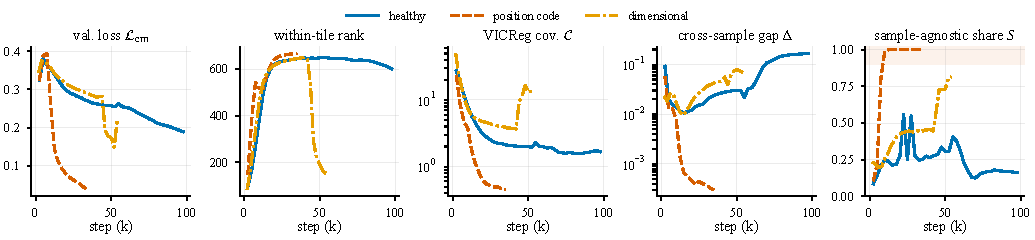
\includegraphics[width=\textwidth]{figures/anatomy.pdf}
  \caption{A healthy run, a position-code collapse and a dimensional collapse (validation curves of runs A1, B1 and D1 in \cref{tab:supp_runs}, which use different recipes). During the position code the loss falls tenfold, the within-tile rank rises and the VICReg covariance drops, all apparent improvements, while the cross-sample gap $\Delta$ goes to zero. In the dimensional collapse the rank falls and the covariance rises, but $\Delta$ increases. Only $S$ (\cref{eq:share}) rises in both; the band marks $S{>}0.9$.}
  \label{fig:anatomy}
\end{figure*}

\subsection{Two failure modes}

\paragraph{Dimensional collapse.} In the run of \cref{fig:anatomy} (fixed-GSD stems, seven products, peak learning rate $10^{-4}$), the effective rank of the target tokens within a tile fell from 651 to 163 between 40k and 52k steps. The VICReg covariance rose from 3.7 to 13.6, the expert load drifted out of balance, and the median gradient norm went from 0.05 to over 200. The validation loss kept falling, from 0.280 to 0.149. This is the dimensional collapse known from joint-embedding methods~\cite{jing2022understanding,hua2021feature}: per-feature variance survives, but the representation concentrates in a few directions. Four of our runs failed this way (\cref{tab:signals}).

\paragraph{Position-code collapse.} The second mode is harder to see. Between 5k and 35k steps of the run in \cref{fig:anatomy}, the validation loss fell from 0.389 to 0.038, the within-tile rank of targets and predictions rose from 382 to 667 and from 160 to 632, and the covariance penalty fell from 8.5 to 0.45. Yet the prediction for a footprint ended with cosine 0.972 to its own target and 0.971 to the target of another footprint. At every cell the model emitted a vector that depended on the cell's position and hardly at all on the terrain. None of its low loss came from content, and every standard signal said the run had improved. Three runs ended this way (\cref{tab:signals}).

\begin{table*}[t]
  \centering
  \small
  \setlength{\tabcolsep}{3.6pt}
  \caption{Common signals while a run fails (runs B1, B2, C2, D1--D3 and E1 in \cref{tab:supp_runs}), from the last healthy validation to the end of the failure. Rank: effective rank of the target tokens within one tile. Colors show what a practitioner would read into each change (\textcolor{ForestGreen}{looks better}, \textcolor{BrickRed}{looks worse}). Only $S$ moves the same, correct way in all seven.}
  \label{tab:signals}
  \begin{tabular}{@{}llccccccc@{}}
    \toprule
    Run & Mode & Steps & Val.\ loss $\mathcal{L}_{\text{obs}}$ & Within-tile rank & VICReg $\mathcal{C}$ & Gap $\Delta$ & Share $S$ \\
    \midrule
    Long-short attention~\cite{zhu2021long} & position    & 5k$\to$35k    & \textcolor{ForestGreen}{.389$\to$.038} & \textcolor{ForestGreen}{382$\to$667} & \textcolor{ForestGreen}{8.5$\to$0.45} & \textcolor{BrickRed}{.013$\to$.0003} & \textcolor{BrickRed}{.22$\to$1.00} \\
    \quad + border clamp                    & position    & 5k$\to$60k    & \textcolor{ForestGreen}{.393$\to$.030} & \textcolor{ForestGreen}{369$\to$665} & \textcolor{ForestGreen}{8.0$\to$0.44} & \textcolor{BrickRed}{.017$\to$.0003} & \textcolor{BrickRed}{.36$\to$1.00} \\
    Standard attn., $w_c{=}0.05$            & position    & 1k$\to$8.5k   & .423$\to$.429                          & \textcolor{ForestGreen}{262$\to$505} & \textcolor{ForestGreen}{3.2$\to$0.26} & \textcolor{BrickRed}{.026$\to$.003}  & \textcolor{BrickRed}{.23$\to$.91} \\
    \midrule
    Fixed-GSD, $S_{\max}{=}600$             & dimensional & 40k$\to$52k   & \textcolor{ForestGreen}{.280$\to$.149} & \textcolor{BrickRed}{651$\to$163}    & \textcolor{BrickRed}{3.7$\to$13.6}    & \textcolor{ForestGreen}{.047$\to$.074} & \textcolor{BrickRed}{.46$\to$.80} \\
    Fixed-GSD, $S_{\max}{=}1000$            & dimensional & 58k$\to$74k   & \textcolor{ForestGreen}{.262$\to$.119} & \textcolor{BrickRed}{625$\to$90}     & \textcolor{BrickRed}{3.2$\to$19.2}    & \textcolor{ForestGreen}{.025$\to$.051} & \textcolor{BrickRed}{.55$\to$.89} \\
    50\% NAC rows                           & dimensional & 25k$\to$92.5k & \textcolor{ForestGreen}{.319$\to$.089} & \textcolor{BrickRed}{628$\to$123}    & \textcolor{BrickRed}{3.2$\to$21.4}    & .026$\to$.024                          & \textcolor{BrickRed}{.29$\to$.96} \\
    Shared-canvas stems                     & dimensional & 27.5k$\to$65k & \textcolor{ForestGreen}{.339$\to$.164} & \textcolor{BrickRed}{623$\to$402}    & \textcolor{BrickRed}{1.4$\to$4.1}     & \textcolor{ForestGreen}{.083$\to$.127} & \textcolor{BrickRed}{.05$\to$.67} \\
    \bottomrule
  \end{tabular}
\end{table*}

\subsection{Why the usual signals are blind}
\label{sec:blind}

Write a target token of product $t$ at cell $i$ of footprint $x$ as
\begin{equation}
  \bar z_t(i, x) = u(i) + m_t + l(\ell_x) + c_t(x, i),
  \label{eq:decomp}
\end{equation}
a position term, a product term, a location term and the rest, which we call content. The predictor gets the first three for free: rotary embeddings give it the query cell, the query carries the target product, and in the earlier recipe the location embedding was added to every token on both paths. Only $c_t$ requires reading the source, and for many product pairs it is barely predictable at the token level (a 100\,m image says little about kilometer-scale roughness). The student can lower the loss on those pairs only by shrinking $c_t$ in its own features, and the EMA target follows. Predicting $u{+}m_t{+}l$ and letting $c_t$ fade is therefore a descent direction. In a same-image JEPA this pull is much weaker, because the context largely determines the masked target~\cite{assran2023self,bardes2024revisiting}. Removing the location embedding from the evidence path (\cref{sec:encoder}) deletes the $l$ term; $u$ and $m_t$ remain, because the predictor must know which cell and which product it is predicting.

This decomposition explains the blind spots in \cref{tab:signals}.
\begin{itemize}[leftmargin=*,itemsep=1pt,topsep=2pt]
  \item \emph{Loss} falls as $c_t$ fades. Whatever cannot be predicted is removed from the target.
  \item \emph{Within-tile rank and token cosine gap} are computed inside one tile, across positions. A position code has $G^2$ distinct tokens per tile, so it scores near the maximum on both.
  \item \emph{VICReg variance}, the per-feature standard deviation over the flattened tokens, is met by $u(i)$ alone.
  \item \emph{VICReg covariance} on flattened tokens is lowest for a position code. In a toy batch of 8 tiles of $64^2$ layer-normalized tokens, a position code scores 0.19. Adding a shared content vector per tile raises it to 8.8, and tokens constant within each tile score 83. The shared per-tile component is what the penalty sees as correlated features. In our runs the collapsed models ended at 0.44--0.45 and the healthy ones at 1.6--2.5.
  \item \emph{Pooled SIGReg}~\cite{balestriero2025lejepa}, applied to the tile-mean prediction $\bar m$, has a scale conflict with \cref{eq:cm}. Layer-normalized tokens give $\|\bar m\|^2 = D\,\bar c$, where $\bar c$ is the mean within-tile cosine. Matching $\mathcal{N}(0, I)$ therefore needs $\bar c \approx 1$, that is, every token in a tile identical. In our runs with SIGReg (weight 0.003) the term sat at a constant ${\approx}67$ ($\bar c{=}0.11$) and pushed only toward smoother tiles.
\end{itemize}
The supplement (\cref{sec:supp_reg}) gives the derivations.

Rotary embeddings are relative, but the design still leaks absolute position. The illumination token sits at a fixed position outside the grid, so a query's attention logit to it depends on the query's absolute cell. At initialization a linear readout of the predictor output recovers the $(\text{row}, \text{col})$ of tokens in a held-out sample with $R^2{=}0.86$ when this token is present (0.20 if the sun differs between samples) and $R^2{=}{-}0.26$ without it. Windowed long-short attention~\cite{zhu2021long} adds a second channel: its zero-padded border windows stamp the window class (corner, edge or interior) onto every token, 2.1 times the noise floor at initialization against 1.2 for standard attention. Both long-short runs in \cref{tab:signals} collapsed as the learning rate approached its peak, the second despite a NATTEN-style border clamp~\cite{hassani2023neighborhood} that cut the stamp to 1.06. The attractor is not specific to that architecture: a standard-attention model with a ten times larger covariance weight reached it within 4k steps.

\subsection{A cross-sample monitor}
\label{sec:monitor}

A position code is invisible within a sample, so we compare across samples. For prediction $\hat z_b$ and target $\bar z_b$ of sample $b$ in a micro-batch, and $\pi(b)$ another sample of the same micro-batch, we log
\begin{align}
  \Delta &= \E_b\big[\cos(\hat z_b, \bar z_b) - \cos(\hat z_b, \bar z_{\pi(b)})\big], \label{eq:gap}\\
  S &= 1 - \Delta \,/\, \E_b\big[\cos(\hat z_b, \bar z_b)\big], \label{eq:share}
\end{align}
where $\cos$ is averaged over the $G^2$ cells and $\bar z$ is layer-normalized. $\Delta$ measures how much better a prediction matches its own footprint than another one, and $S$ is the share of the agreement that another footprint's target would have received anyway. A position code gives $\Delta\to0$ and $S\to1$. Dimensional collapse makes all targets alike, so the cosine grows faster than the gap and $S$ rises even while $\Delta$ increases (\cref{tab:signals}). The cost is one extra cosine per target.

$S$ passed 0.65 in all seven failures and 0.8 in six of them. It is not a clean threshold. Runs that stayed useful ended between 0.16 and 0.57, but three of them passed 0.69--0.74 for a validation or two (\cref{tab:supp_runs}). We read $S{<}0.35$ as healthy and $S{>}0.9$ as collapsed; in between, we watch whether $\Delta$ is still rising. For position codes, $S$ gave the earliest warning. It passed 0.7 at 7.5k steps, when the loss had not yet moved and the within-tile token cosine gap was still 0.06.

The monitor has limits. $\Delta$ rewards anything that differs between footprints, including the location term $l$ and, when $\pi(b)$ holds a different product, the product term, so a code built from $u$, $m_t$ and $l$ would pass. It cannot see predictions that stay specific to the footprint but lose detail within the tile. In one run the within-tile token cosine gap fell from 0.015 to 0.006 between 32.5k and 67.5k steps while $\Delta$ held at 0.03--0.05, so we log both kinds of monitor. $\Delta$ is identically zero at micro-batch size one, and it is measured against each run's own EMA target, so absolute values compare only runs whose targets are alike. It is an alarm and a within-recipe score, not a substitute for downstream evaluation.

\paragraph{A timing trap.} $\Delta$ starts high (0.1--0.4 in the first 1--2k steps), because the targets of a fresh encoder are easy to tell apart, and then falls several-fold, with the variance hinge within a few hundred steps of the prediction standard deviation snapping to 1 (\cref{sec:ablations}). Runs must be compared after this trough, at matched steps.

\section{Experiments}
\label{sec:experiments}

\paragraph{Setup.} The encoder has 217M parameters (104M active per token) and the predictor 116M. The stems add 1.7M (linear) to 62M (convolutional) parameters over all product slots. We use AdamW~\cite{loshchilov2019decoupled} (weight decay 0.05, clipping at 1), bf16, linear warmup over 10\% of the steps and cosine decay, on 16--64 A100 GPUs with 96 to 3072 footprint rows per step and flash attention~\cite{dao2022flashattention} at $G{\geq}64$. Every 2.5k steps we validate on a fixed, seeded subset of the validation footprints with the block mask applied. All runs reported here use the single-observation configuration of \cref{sec:objective} ($K{=}1$, no state head, location embedding on all tokens, VICReg on evidence and predictions). Recipes changed as the project went on, so each comparison below changes one setting of one recipe (\cref{sec:supp_runs}), and all results are single runs. \TODO{multi-observation and state-head runs; see the planned experiments below}

\subsection{What pushes a run toward collapse}
\label{sec:ablations}

\begin{table}[t]
  \centering
  \footnotesize
  \setlength{\tabcolsep}{2.5pt}
  \caption{One-variable comparisons: $\Delta$ and $S$ at the same step in both arms. Background recipes differ between rows; the runs are listed in \cref{tab:supp_runs}. $^\dagger$The shared-canvas arm collapsed at this step and diverged shortly after; the fixed-GSD arm trained stably to 82.5k ($\Delta{=}0.060$, $S{=}0.38$).}
  \label{tab:ablations}
  \begin{tabular}{@{}lrcc@{}}
    \toprule
    Change (baseline $\to$ variant) & Step & $\Delta$ & $S$ \\
    \midrule
    Hinge on $\hat z$: $\gamma{=}1\to$ off        & 10k   & .010 $\to$ .055 & .77 $\to$ .24 \\
    Hinge on $\hat z$: $\gamma{=}1\to0.3$         & 2.5k  & .021 $\to$ .033 & .39 $\to$ .30 \\
    Covariance $w_c$: $0.005\to0.05$              & 8k    & .204 $\to$ .003 & .38 $\to$ .90 \\
    4 MoE layers $\to$ dense                      & 97.5k & .167 $\to$ .094 & .16 $\to$ .52 \\
    Kernel floor $k_{\min}$: $1\to4$              & 97.5k & .167 $\to$ .121 & .16 $\to$ .25 \\
    Shared canvas $\to$ fixed-GSD$^\dagger$       & 65k   & .127 $\to$ .045 & .67 $\to$ .56 \\
    Grid $G$: $64\to32$                           & 10k   & .010 $\to$ .009 & .77 $\to$ .55 \\
    Grid $G$: $64\to128$                          & 10k   & .010 $\to$ .016 & .77 $\to$ .63 \\
    \bottomrule
  \end{tabular}
\end{table}

\begin{figure*}[t]
  \centering
  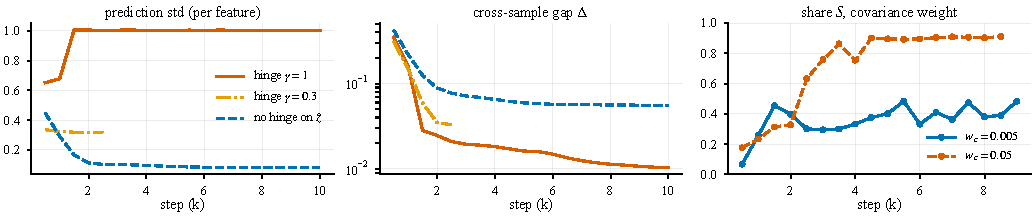
\includegraphics[width=\textwidth]{figures/regularizers.pdf}
  \caption{Two regularizers that pull the wrong way. \emph{Left, middle:} with the variance hinge on the predictions ($\gamma{=}1$), their per-feature standard deviation jumps to 1 at 1.5k steps and $\Delta$ drops fivefold within 500 steps. Without it, the standard deviation settles near 0.08 and $\Delta$ ends 5.3 times higher. The $\gamma{=}0.3$ run stopped early. \emph{Right:} a covariance weight of 0.05 sends a standard-attention model into a position code by 4k steps.}
  \label{fig:regularizers}
\end{figure*}

\paragraph{The variance hinge fights calibration.} The VICReg variance term asks for a per-feature standard deviation of at least $\gamma$ across tokens. That sounds harmless for layer-normalized targets, but a calibrated prediction $\E[\bar z\mid\text{source}]$ has a standard deviation of about $\sqrt{R^2}$, where $R^2$ is the share of the target's variance the source explains. Ours is around 1\%, so the hinge asks for ten times the calibrated spread. The cheapest variance to add without raising the loss is structure that the target also has and the predictor can produce without reading the source: $u$, $m_t$ and $l$ of \cref{eq:decomp}. With the hinge, the prediction standard deviation snaps to 1 and $\Delta$ drops fivefold within 500 steps (\cref{fig:regularizers}). Turning it off for the predictions (it stays on the evidence) gives 5.3 times the gap at 10k steps, $S$ of 0.24 instead of 0.77 and a lower validation loss (0.350 vs.\ 0.390), and $\gamma{=}0.3$ falls in between. The hinge is on in every other run in this paper, including the downstream backbone, and probably explains part of their early trough. In the recipe of \cref{sec:objective} the hinge acts only on the state head.

\paragraph{Covariance and experts.} Raising $w_c$ from 0.005 to 0.05 turned a standard-attention model into a position code within 4k steps, as \cref{sec:blind} predicts. Removing the four MoE layers lowered the late gap from 0.167 to 0.094 and raised $S$ from 0.16 to 0.52, while the validation loss improved (0.168 vs.\ 0.189). The routers were not trouble-free: in three long runs the first MoE layer lost balance before the gradient norm grew, and one run ended with three quarters of its experts unused.

\subsection{Tokenization}
\label{sec:exp_tokens}

\paragraph{Fixed-GSD stems vs.\ a shared canvas.} With five products and nothing else changed, the shared-canvas model reached the higher gap (0.169 at 55k steps) but then collapsed dimensionally (rank 623 $\to$ 402) and diverged at 66k. The fixed-GSD model held its rank near 610 and trained stably to the end of its allocation at 82.5k. The two stems produce different targets, so their gap values are not comparable; their stability is.

\paragraph{Kernel floor.} The floor does what it was meant to do (\cref{tab:floor}). With $k_{\min}{=}1$, pairs involving LOLA roughness were close to chance ($\Delta{=}0.033$ as target, 0.023 as source). With $k_{\min}{=}4$ they rose three- to fourfold, and TiO$_2$ gained as a target. The other pairs lost ground (0.205 $\to$ 0.122), and so did the overall gap. With one seed per arm we cannot tell a trade-off from run-to-run variation.

\paragraph{Grid size.} In a 10k-step sweep that changed only $G$, the validation loss improved with resolution (0.420, 0.390, 0.364 for $G{=}32, 64, 128$), and $G{=}128$ ended with the largest training-window gap on 11 of 12 target products. On 32 GPUs the runs took 24, 28 and 63 hours. All three had the variance hinge on and ended in the trough of \cref{sec:monitor}, so the numbers rank the grids but understate them. We use $G{=}64$ as the compromise.

\paragraph{Dense-prediction upgrades.} The dense context loss (\cref{eq:ctx}) and the convolutional stems both aim at better features per cell. Trained together at $G{=}32$ with shared-canvas stems and seven products, they raised $\Delta$ from 0.19 at the first validation (2.5k steps) to 0.308 at 10k instead of dropping into the trough, and held 0.294 at 35k, with $S$ between 0.05 and 0.23. The closest earlier run shares grid, products, learning rate, batch and regularizers and reached $\Delta{=}0.064$ ($S{=}0.45$) at 35k; it differs in normalization statistics, validation subset and code version, so the comparison is confounded. \TODO{clean ablation with both upgrades off, and the $G{=}64$ runs on both stem types}

\subsection{Downstream}
\label{sec:downstream}

The downstream results use an earlier checkpoint ($G{=}64$, shared-canvas stems, six products, 79k steps at a peak learning rate of $10^{-4}$, variance hinge on). Its transformer is always frozen. The crater detectors fine-tune the per-product stems with their heads, and the probes read frozen features only (\cref{sec:supp_downstream}).

\begin{table}[t]
  \centering
  \footnotesize
  \setlength{\tabcolsep}{3.5pt}
  \caption{Crater detection with a frozen encoder and fine-tuned stems (test split, single seed). \emph{Top:} FCOS heads~\cite{tian2019fcos} with our neck. \emph{Bottom:} the NASA-IBM LFM protocol (Faster R-CNN family, WAC only, boxes of at least 10\,px, at most 500 detections).}
  \label{tab:craters}
  \begin{tabular}{@{}llcc@{}}
    \toprule
    Data & Input & mAP$_{50}$ & mAP \\
    \midrule
    Robbins, 1k tiles  & WAC                     & 0.530 & 0.238 \\
                       & WAC + predicted DTM     & 0.549 & 0.242 \\
                       & WAC + DTM               & 0.595 & 0.285 \\
    Robbins, 10k tiles & WAC                     & 0.530 & 0.270 \\
                       & WAC + DTM               & \textbf{0.755} & \textbf{0.411} \\
    NAC, hand-labeled  & NAC                     & 0.690 & 0.319 \\
    \midrule
    \multicolumn{2}{@{}l}{NASA-IBM LFM~\cite{fraccaro2026multimodal}, our reproduction} & 0.464 & 0.190 \\
    \multicolumn{2}{@{}l}{Ours, LFM detection stack}                  & 0.362 & 0.156 \\
    \multicolumn{2}{@{}l}{Ours, our neck + jitter, tokens only}       & 0.433 & 0.187 \\
    \multicolumn{2}{@{}l}{Ours, our neck + jitter + pixel branch}     & \textbf{0.494} & \textbf{0.217} \\
    \bottomrule
  \end{tabular}
\end{table}

\paragraph{Crater detection.} We train detection heads for the Robbins catalog~\cite{robbins2019new} on WAC tiles at 100\,m (1k and 10k tiles) and for hand-labeled NAC craters at 0.8--5\,m from six of the ten NAC photometry sites of SomBench~\cite{patil2026sombench} (\cref{tab:craters}). Adding the DTM as a second input to the same frozen backbone is the largest single effect: $+0.065$ mAP$_{50}$ with 1k tiles and $+0.225$ with 10k tiles, where the lighting varies more. A DTM that the backbone itself predicts from the WAC image recovers 0.019 of the 0.065. For a comparison with the NASA-IBM lunar foundation model~\cite{fraccaro2026multimodal}, which is trained by masked token prediction, we reproduced its frozen-backbone Faster R-CNN protocol on the same data and obtained 0.464 mAP$_{50}$ for that model, against 0.458 reported. With its detection stack our tokens reach 0.362--0.390. With our neck and scale jitter they reach 0.433 from tokens alone, and 0.494 when the detector also gets a raw-pixel branch. Our fine-tuned stems favor us in this comparison, so we read it as rough parity on single-product craters. The distinctive gain comes from the second product.

\paragraph{Shape, albedo and shadows.} A WAC image mixes topography, albedo and illumination, and the backbone was never trained to separate them. We probe whether its predictions do, on 40 held-out footprints seen under eight suns each (all metrics in \cref{tab:safs}). Given only a WAC image, linear probes on the predictor features for the elevation and 643\,nm products recover relief with correlation 0.705 (0.12 for the same probe on pixels) and albedo with 0.840. Both barely change with the sun, and the predicted relief picks the right footprint among the 40 in 96\% of cases. A small head that integrates the backbone's own slope and aspect predictions reaches a relief RMSE of 299\,m (551\,m for zero relief). The reverse direction tests the sun conditioning. From topography and a sun, a linear probe on the predictor's WAC features localizes cast shadows with AUC 0.89, against 0.59 with another observation's sun and 0.49 with none. The predictor uses the sun it is given.

\subsection{Planned experiments}
\label{sec:planned}

The recipe of \cref{sec:method} is being trained on the corpus of \cref{sec:dataset}; the comparisons below are designed, and their tables will replace the TODOs. \emph{(E1) Observations and state.} At matched budget, $K{=}1$ without the state head (the configuration above) against $K\in\{1,2,3\}$ with it, scored by $\Delta$, by the content and position probes of \cref{sec:supp_runs}, and by the downstream tasks. \emph{(E2) Relighting.} The repeat-acquisition task on and off, scored by the sun-swap shadow test and by how much the state $\hat w$ of one footprint changes between its observations. \emph{(E3) Location.} The location embedding on all tokens, on the predictor only with dropout, and absent, to measure how much of $\Delta$ the $l$ term of \cref{eq:decomp} accounts for. \emph{(E4) Monitors.} Over all checkpoints, each monitor as a detector of the probe labels, with AUROC and lead time. \emph{(E5) Baselines.} The NASA-IBM model~\cite{fraccaro2026multimodal}, DINOv3~\cite{simeoni2026dinov3} and a random encoder on crater detection, irregular mare patch segmentation~\cite{braden2014evidence,patil2026sombench} and polar ice prospectivity, with LunarFM~\cite{gironamata2026lunarfm} and Moonstone~\cite{prasad2026moonstone} where weights are available.

\section{Limitations and Conclusion}
\label{sec:conclusion}

\paragraph{Limitations.} All comparisons are single runs, and several change one setting on top of recipes that differ from each other. The downstream backbone predates the fixed-GSD stems, the dense context loss, the convolutional stems, the multi-observation encoder and the state head, so the recipe of \cref{sec:method} is not yet evaluated downstream. The cross-sample gap cannot separate content from location or product identity, and it compares only runs whose targets are alike. The mechanism of \cref{eq:decomp} is supported by probes and ablations but not proven. The corpus counts predate the seam repair, and polar footprints and the 1\,m NAC scale, where much of the scientific demand lies, are outside the runs reported here.

\paragraph{Conclusion.} After the raw products are calibrated and projected, the lunar archive becomes a dataset only once they are cut to common ground, and we described a pipeline that does this at the scale of the whole Moon while keeping every camera observation of a footprint, with its geometry, rather than one view per tile. On this corpus, predicting one instrument from another in latent space, under the sun of the target, is a workable pretraining task. Its frozen features detect craters about as well as a masked-token lunar model, gain substantially from a second product and respond to the sun they are given. Getting there taught us more about failure than about architecture. A cross-modal JEPA can reach a very low loss by encoding where a token is instead of what the ground looks like, and loss, within-sample rank and VICReg all read this as progress. A cross-sample comparison exposes it for one cosine per target, and we would log it in any JEPA whose targets are only partly predictable from the context.

{
    \small
    \bibliographystyle{ieeenat_fullname}
    \bibliography{main}
}

% WARNING: remove the supplementary pages from the main submission.
\clearpage
\setcounter{page}{1}
\maketitlesupplementary
\appendix

\section{Corpus details}
\label{sec:supp_data}

This section is the long form of \cref{sec:dataset}. Raw records, their calibration and orthorectification, and the selection of WAC and NAC records are shared with SomBench~\cite{patil2026sombench}; everything below the preprocessed products (the footprint grid, attachment of every layer, repeat observations on identical bounds, the sub-tile level, seam ownership, catalogs and splits) is specific to this corpus.

\begin{table*}[t]
  \centering
  \scriptsize
  \setlength{\tabcolsep}{3pt}
  \caption{All 34 layers of the corpus. Per-image products carry acquisition geometry and appear once per observation; static layers appear once per footprint. Polar layers exist only on the two polar caps. $r$: native resolution. Tile: pixels per side of a 60\,km footprint, $\lfloor 60\,\text{km}/r \rfloor$; for NAC and terrain, pixels per side of a 500\,m sub-tile. NaN\%: fraction of missing pixels, measured over every pixel of the released tiles (radar: reflectivity / CPR; WAC is zero by construction, since records with any missing pixel are rejected). Diviner bolometric temperature and GRAIL gravity are $4\times4$ and $3\times3$ rasters per footprint and are used only as coarse conditioning. Extent gives the latitude range of the source product.}
  \label{tab:layers}
  \resizebox{\textwidth}{!}{%
  \begin{tabular}{@{}llrrllrl@{}}
    \toprule
    Layer & Instrument / mission & $r$ (m) & Tile & Bands & Extent & NaN\% & Ref. \\
    \midrule
    \multicolumn{8}{@{}l}{\emph{Per-image (footprints)}} \\
    WAC visible & LRO LROC WAC & 100 & 600 & 415, 566, 604, 643, 689\,nm & global & 0.0 & \cite{robinson2010lunar,mahanti2016inflight} \\
    WAC ultraviolet & LRO LROC WAC & 500 & 120 & 321, 360\,nm & global & 0.0 & \cite{robinson2010lunar} \\
    \multicolumn{8}{@{}l}{\emph{Per-image (sub-tiles)}} \\
    NAC panchromatic & LRO LROC NAC & $\approx$1 & 500 & I/F & where imaged & 10.3 & \cite{robinson2010lunar,humm2016flight} \\
    NAC stereo terrain & LROC NAC DTMs & 3 & 166 & elevation, slope, aspect (sin, cos) & DTM sites & 5.0 & \cite{henriksen2017extracting} \\
    \midrule
    \multicolumn{8}{@{}l}{\emph{Static, equatorial and shared (16)}} \\
    Topography & SLDEM2015 (LOLA + Kaguya TC); LOLA polar & 60 & 1000 & elevation, slope, aspect (sin, cos) & global & 0.0 & \cite{barker2016new,barker2023new} \\
    Roughness & LOLA & 1000 & 60 & 50\,m-baseline roughness & global & 13.0 & \cite{kreslavsky2013lunar,neumann2015copernican} \\
    Morphologic mosaic & LROC WAC (643\,nm, high incidence) & 100 & 600 & 1 & global & 0.0 & \cite{speyerer2011lunar,wagner2015new} \\
    643\,nm normalized mosaic & LROC WAC, empirical photometric model & 100 & 600 & 1 & global & 0.26 & \cite{boyd2012lunar} \\
    Normalized reflectance & LROC WAC & 500 & 120 & 321--689\,nm (7) & $60^\circ$S--$60^\circ$N & 13.2 & \cite{boyd2012lunar} \\
    TiO$_2$ & LROC WAC (321/415\,nm ratio) & 400 & 150 & wt\% & $70^\circ$S--$70^\circ$N & 4.7 & \cite{sato2017lunar} \\
    MI reflectance & Kaguya Multiband Imager & 60 & 1000 & 414--1548\,nm (8) & $55^\circ$S--$55^\circ$N & 10.6 & \cite{ohtake2008performance,lemelin2016global} \\
    MI mineralogy & Kaguya MI inversion & 60 & 1000 & CPX, OPX, olivine, plag., grain size, FeO, OMAT & $50^\circ$S--$50^\circ$N & 23.4 & \cite{lemelin2015lunar,lemelin2016global} \\
    MI space weathering & Kaguya MI radiative transfer & 1000 & 60 & smFe, mpFe, npFe & $55^\circ$S--$55^\circ$N & 14.3 & \cite{trang2019improved} \\
    Rock abundance & LRO Diviner & 240 & 250 & areal fraction & $70^\circ$S--$70^\circ$N & 5.1 & \cite{powell2023high} \\
    Regolith temperature anomaly & LRO Diviner & 240 & 250 & K & $70^\circ$S--$70^\circ$N & 5.1 & \cite{powell2023high} \\
    H-parameter & LRO Diviner & 240 & 250 & m & $70^\circ$S--$70^\circ$N & 5.5 & \cite{hayne2017global} \\
    Radar & LRO Mini-RF (S-band) & 90 & 666 & S1 reflectivity, CPR & global & 42.5 / 43.5 & \cite{nozette2010lunar,fassett2024improved} \\
    Geologic map & USGS unified map & 60 & 1000 & 43 units (categorical) & global & 0.0 & \cite{fortezzo2020release} \\
    Bolometric temperature & LRO Diviner & 15000 & 4 & 24 local-time bins & global & 0.0 & \cite{williams2017global} \\
    Free-air gravity & GRAIL & 20000 & 3 & mGal & global & 0.0 & \cite{zuber2013gravity} \\
    \midrule
    \multicolumn{8}{@{}l}{\emph{Static, polar (14)}} \\
    Summer / winter temperature & LRO Diviner & 240 & 250 & 24 bins each (2 layers) & $80$--$90^\circ$ & $\approx$3 & \cite{williams2019seasonal} \\
    Ice stability depth & LRO Diviner + thermal model & 240 & 250 & m & $80$--$90^\circ$ & 27.4 & \cite{schorghofer2020mapping} \\
    Average illumination & LOLA DEM horizon model & 120 & 500 & fraction & $75$--$90^\circ$ & 0.0 & \cite{mazarico2011illumination} \\
    Permanently shadowed regions & LOLA DEM & 20 & 3000 & mask & $80$--$90^\circ$ & 0.0 & \cite{mazarico2011illumination,barker2023new} \\
    1064\,nm normal albedo & LOLA & 1000 & 60 & 1 & $50$--$90^\circ$ & 0.0 & \cite{lemelin2016improved} \\
    SP mineralogy & Kaguya Spectral Profiler & 1000 & 60 & olivine, plag., HCP, LCP, npFe, FeO, OMAT (7 layers) & $80$--$90^\circ$ & 4.3 & \cite{lemelin2022compositional} \\
    Hydrogen abundance & Lunar Prospector NS & 15000 & 4 & ppm & $60$--$90^\circ$ & 0.0 & \cite{lawrence2022global} \\
    \bottomrule
  \end{tabular}}
\end{table*}

\paragraph{Layers.} \Cref{tab:layers} lists the 34 layers: four per-image products (WAC visible and ultraviolet on the footprints, NAC panchromatic and NAC stereo terrain on the sub-tiles) and 30 static layers. Sixteen static layers cover the equatorial strips, and those whose source reaches the poles are also extracted on the caps; fourteen exist only on the caps. Static layers are present on 10,525 equatorial and 104 polar footprints. Every per-image record keeps the geometry of its acquisition (incidence, emission and phase angles, sub-solar ground azimuth, sub-solar and sub-spacecraft latitude and longitude, north azimuth), which conditions the predictor when the record is a target. Diviner bolometric temperature and GRAIL gravity hold only $4\times4$ and $3\times3$ pixels per footprint; they serve only as coarse conditioning and are not among the products of \cref{tab:modalities}. Any other layer can act as source or target.

\paragraph{Regions and projections.} Equatorial footprints live in one of 90 Lunar Transverse Mercator strips~\cite{mcclernan2025lunar}, 45 zones of $8^\circ$ longitude per hemisphere covering $|\phi| \le 82^\circ$; polar footprints live in a north or south polar stereographic cap covering $|\phi| \ge 82^\circ$. A footprint is a $3\times3$ block of GRAIL pixels, $60\times60$\,km in the projection of its region, and footprints are laid with a stride equal to their size. The footprint size must be an integer multiple of the 20\,km GRAIL pixel, so the master grid is never resampled. We use no overlap: two overlapping footprints would store pixel-identical static content over their intersection, the same WAC record would be clipped twice with the same acquisition geometry, so diversity sampling could not turn the duplicate into a new view, and each sub-tile under $m$ parents would be materialized $m$ times. Zones 1 and 45 are inset by $0.5^\circ$ from $\pm180^\circ$ to avoid warp artifacts of the virtual rasters at the discontinuity, footprints whose four-corner envelope spans more than $180^\circ$ of longitude are skipped, and whole zones can be excluded by configuration (off by default). Spatial matching of camera records to footprints is done in lunar geographic coordinates (IAU\_2015:30100) for the strips, where a footprint is a faithful box and the same index serves every strip. On the caps matching is done in projected coordinates, because a 60\,km square near the pole unprojects to a longitude range of hundreds of degrees, which no single swath can contain; records whose footprints become invalid or empty under projection to the cap, typically those from the opposite pole, are dropped when the index is built. A projection-compatibility checker rejects impossible source and target pairs, such as a polar stereographic record against a strip footprint, before any pixel is read.

\paragraph{Static-map extraction.} For each strip or cap, the GRAIL virtual raster cropped to the region defines the footprint centers and bounds, and every static layer is then read lazily from the region's virtual raster, which already holds it in the footprint's projection. Each layer is clipped to the footprint bounds at its native pixels, giving $t = \lfloor 60\,\text{km}/r \rfloor$ pixels per side (\cref{tab:layers}), from 1000 for SLDEM2015 to 3 for GRAIL; there is no reprojection and no snapping of the resolution at this stage. Layers whose source pixels do not align with the footprint origin, GRAIL and Diviner bolometric temperature, are resampled within the same projection to restore the exact $t\times t$ shape. Bands are stacked with their names, so a multi-band layer such as the eight MI reflectance bands stays addressable by wavelength. Each static layer is extracted once per footprint and shared by all WAC observations of that footprint and all NAC and terrain tiles of its sub-tiles. The image-anchored layout of SomBench instead re-clips every static layer for every image tile, which takes 21.5\,M netCDF files and 42.5\,TB against 9.5\,TB here. The polar registry adds the polar-only layers and polar projections of the shared ones; both registries emit catalogs with the same columns.

\paragraph{Per-image extraction.} Camera records are orthorectified products of~\cite{patil2026sombench}, each projected into the strip, or cap, that holds the largest fraction of its area, so a record can extend into neighboring strips. The WAC candidates of a footprint are the records whose geodatabase footprint polygons contain it, with incidence, emission and phase in $[0, 90]^\circ$ and sub-solar ground azimuth in $[0, 360]^\circ$; the pool holds 59,503 WAC products on disk. Extraction follows three rules. (i) Matching is done in geographic coordinates, or in projected ones on the caps (\cref{sec:grid}). (ii) A record whose strip equals the footprint's strip is sliced directly; otherwise the clip is cut in the record's own projection and only the clip is reprojected. The four footprint corners are transformed into the record's projection, the clip is enlarged by a 2-pixel buffer without resampling, reprojected to the footprint's projection and trimmed symmetrically, so no boundary pixel comes from edge padding. (iii) Every box transformed between projections uses the envelope of all four transformed corners, since the two-corner $(\min, \max)$ shortcut can swap the ordering of $x$ or $y$ under a nonlinear projection and silently truncate the footprint.

Two samplers select at most $k{=}500$ records per footprint. The default diversity-binned sampler places candidates on a two-dimensional illumination grid of 20 uniform incidence bins and $\operatorname{round}(k/20){=}25$ uniform sub-solar ground azimuth bins, with bin edges computed once per strip from the observed metadata range. Candidates are ordered by a randomized round-robin over occupied cells and extracted under a budget of five attempts per retained slot; the final selection again round-robins over cells, taking the lowest-NaN candidate within each cell first, so the kept set spans the available suns instead of collapsing onto the $k$ best-covered records, which are often near-duplicates. A record with any missing visible or ultraviolet pixel is rejected and the sampler continues down its ordering. Retained records are stored sorted by NaN fraction, so rank 0 is the best-covered observation. The alternative coverage-ranked sampler orders candidates by a 5:2 weighted mean of visible and ultraviolet NaN fraction and keeps the $k$ best, stopping early once $k$ complete records are found. Visible tiles have shape $(5, 600, 600)$ at 100\,m and ultraviolet tiles $(2, 120, 120)$ at 500\,m, and each record keeps its acquisition geometry, its rank and its combined NaN percentage. The result is 476,635 WAC records over 10,629 footprints; 9,232 footprints (86.9\%) have at least one, with 51.6 records per covered footprint on average (\cref{fig:illum}). This stack of co-registered images of the same ground under different suns is the supervision \method relies on.

\begin{figure}[t]
  \centering
  \begin{subfigure}[t]{0.49\linewidth}
    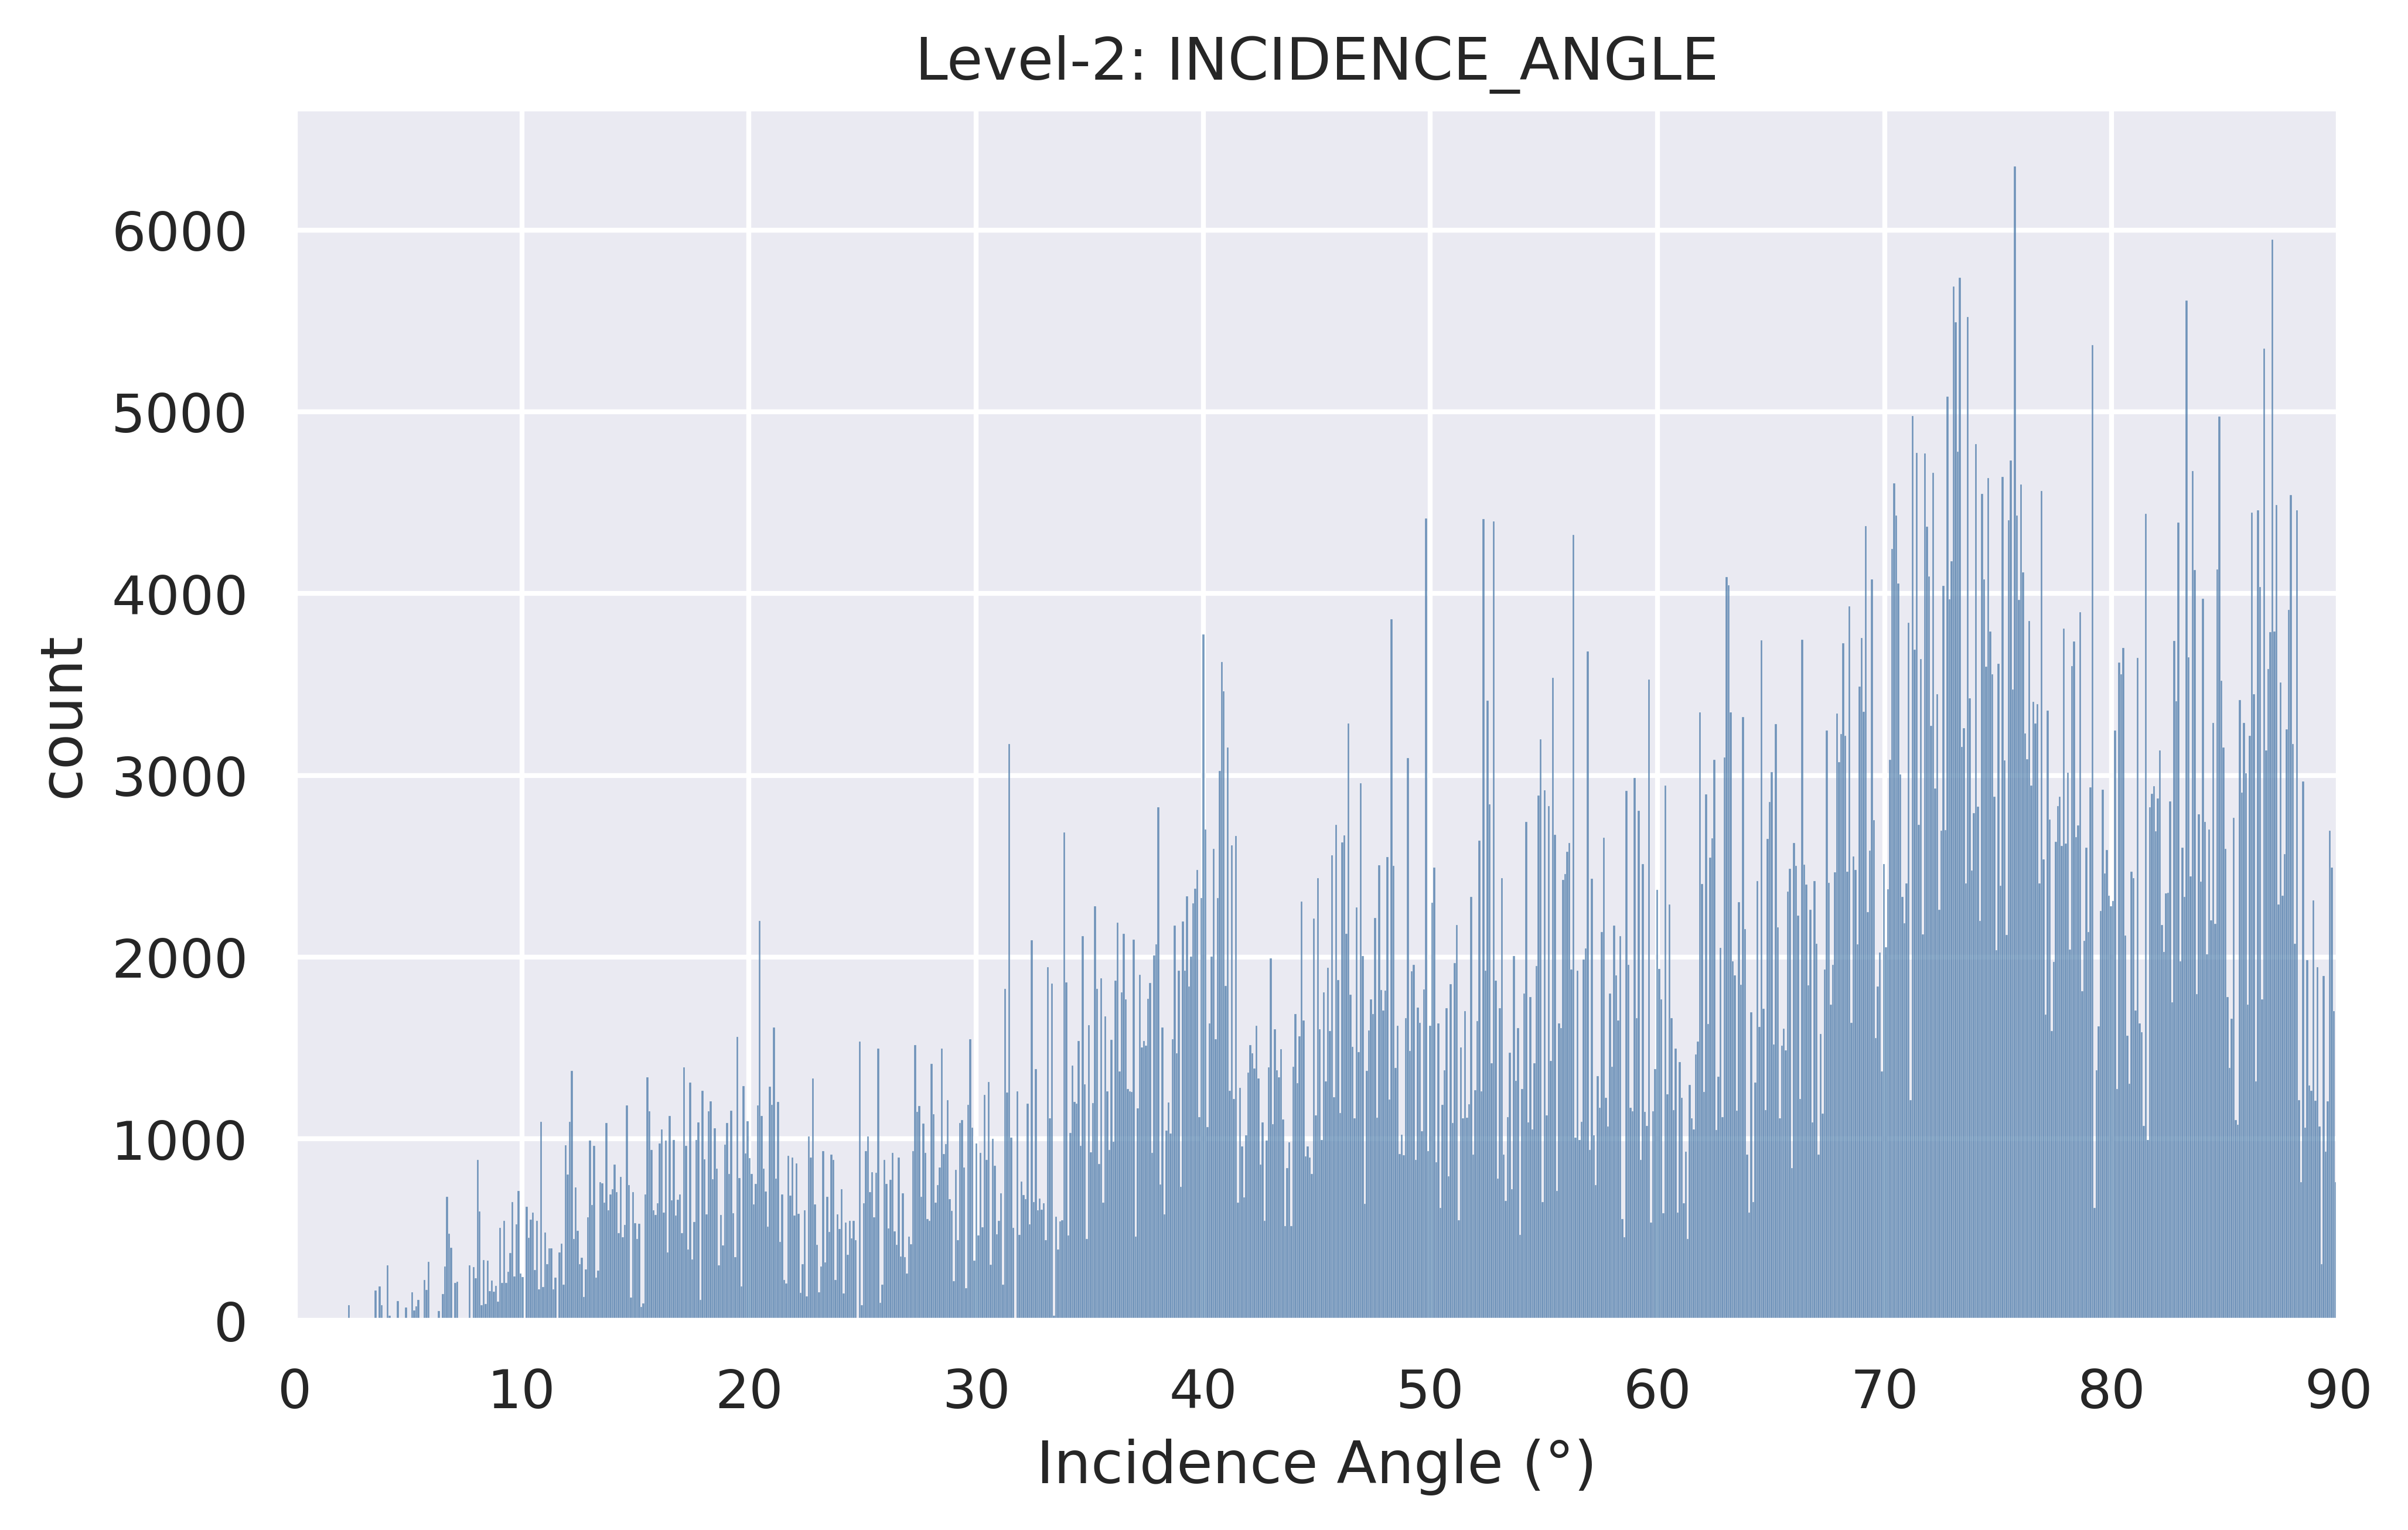
\includegraphics[width=\linewidth]{figures/level2_INCIDENCE_ANGLE.png}
    \caption{Incidence angle.}
  \end{subfigure}\hfill
  \begin{subfigure}[t]{0.49\linewidth}
    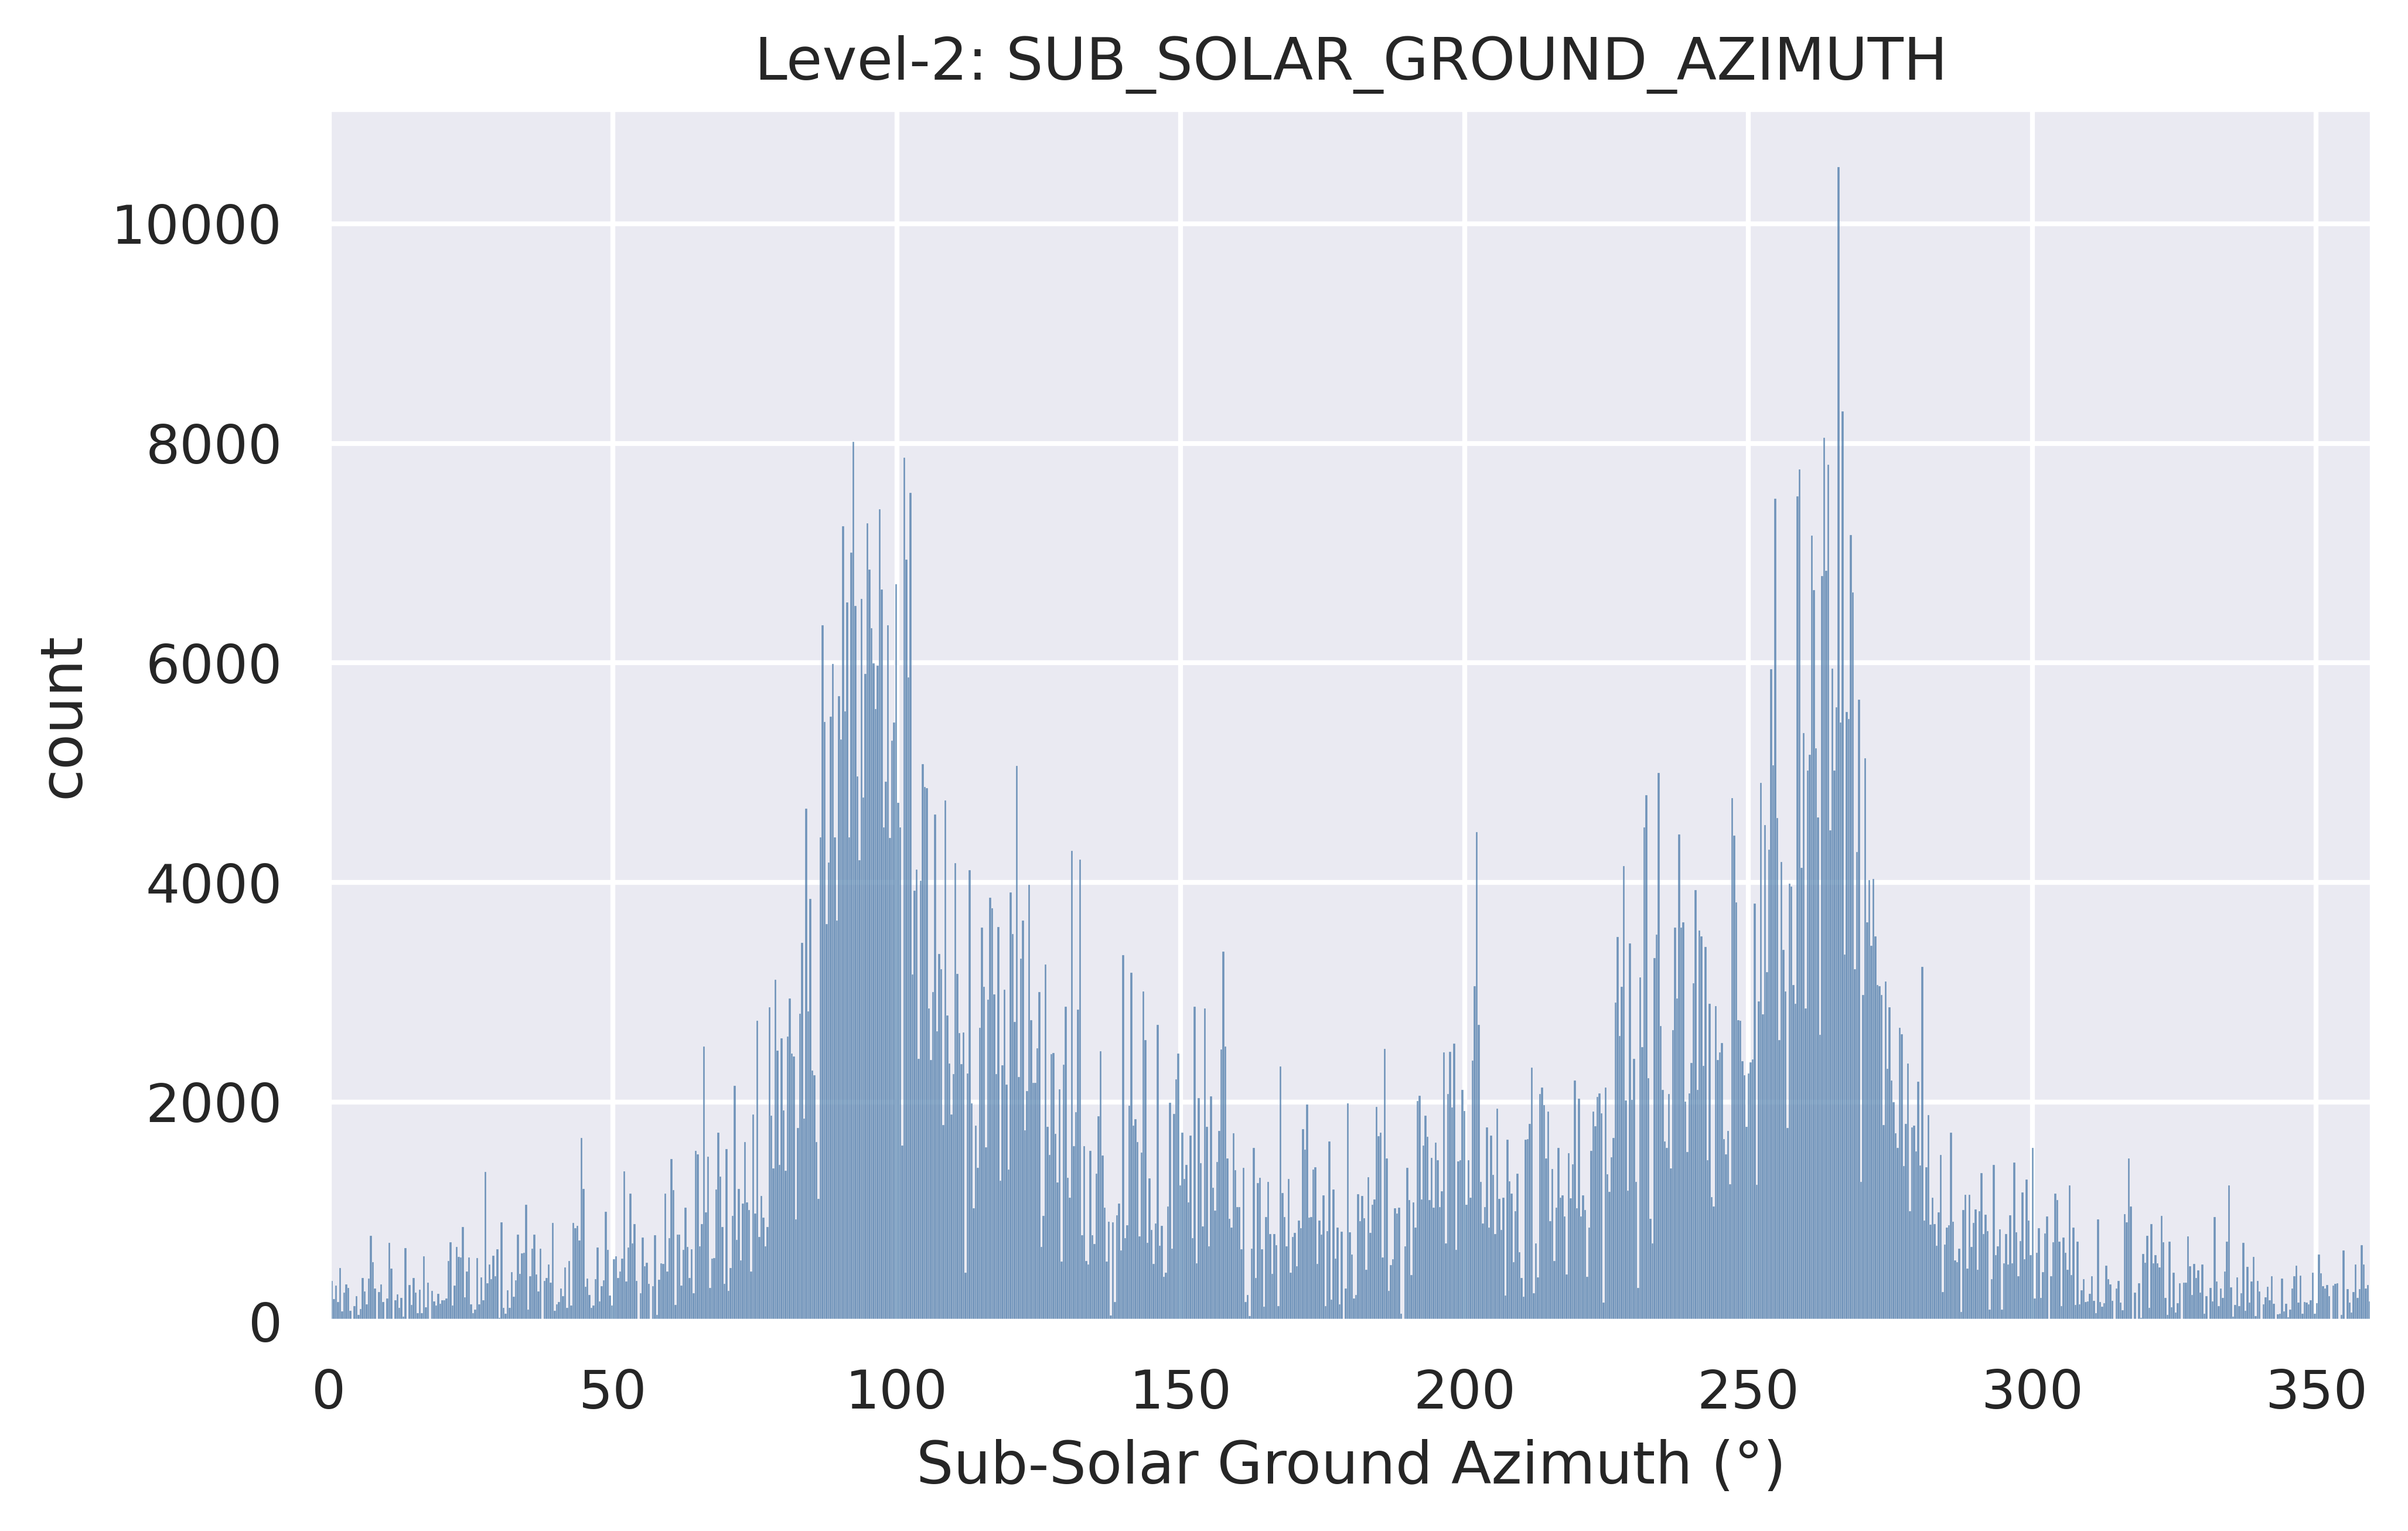
\includegraphics[width=\linewidth]{figures/level2_SUB_SOLAR_GROUND_AZIMUTH.png}
    \caption{Sub-solar ground azimuth.}
  \end{subfigure}
  \caption{Illumination of the NAC records retained over all 500\,m sub-tiles. The same diversity-binned sampler as for WAC bins each sub-tile's candidates on 20 incidence and 25 azimuth bins and fills the cells round-robin, lowest NaN first, up to $k{=}500$. The retained records spread over incidence up to $90^\circ$; the two azimuth peaks are inherited from the pool, since the sampler can only redistribute the geometries that a sub-tile's candidates offer.}
  \label{fig:illum_nac}
\end{figure}

\paragraph{Level 2.} NAC at about 1\,m on a 60\,km footprint would be 60,000 pixels per side ($3.6\times10^9$ cells per band), stereo terrain at 3\,m 20,000, and a NAC swath covers only a fraction of a footprint, so a footprint-sized canvas would be mostly missing. Each footprint is therefore divided into $120\times120$ sub-tiles of 500\,m (14,400 per parent) by the same grid generator, with geographic bounds from the four-corner envelope, an identifier that is a deterministic function of the sub-tile centroid and the parent, and a parent key. This step writes geometry and scalars only. A vectorized spatial join against the NAC and terrain footprint indexes drops sub-tiles with no candidate record and keeps per-source candidate flags; after extraction, sub-tiles with neither NAC nor terrain are pruned. Every static band of the parent is read once through a windowed, average-resampled read and reduced to a per-sub-tile mean (41 bands in the equatorial registry, 71 in the polar one; for maps coarser than the sub-tile this is the covering pixel), so a sub-tile carries its parent's state as scalars without a join.

NAC records are selected with the same diversity-binned sampler and $k{=}500$, ranked by NaN fraction (\cref{fig:illum_nac}). A record that covers only part of a sub-tile is placed at its true geographic offset in a $500\times500$ canvas filled with NaN, and canvases more than 99\% missing are never written; NAC tiles have shape $(1, 500, 500)$. Opening every matched record for every sub-tile would take about $5\times10^8$ clip-and-reproject operations. Extraction is instead batched by parent: each matched record is opened once per parent, a first pass computes the valid-pixel count of every sub-tile from an integral image of the reprojected record without materializing any canvas, the top-$k$ selection is made from these counts, and a second pass materializes only the selected (sub-tile, record) pairs. Reprojected arrays are processed in memory-bounded chunks, falling back to row strips for large records, and per-parent checkpoints make a strip resumable. Stereo terrain has five bands (elevation, slope, aspect and its sine and cosine); each sub-tile keeps the single record with the lowest elevation NaN fraction, under the same 99\% gate evaluated on elevation, as a $(5, 166, 166)$ tile. Eight equatorial strips intersect no terrain model at all (LTM 2N, 9N, 12N, 40N, 16S, 24S, 33S and 37S). The sub-tile level holds 5,354,773 sub-tiles with NAC or terrain, 9,453,706 NAC records after the exclusion of defective products (9,455,461 before), and 856,535 terrain records; 86.6\% of sub-tiles have NAC and 16.0\% terrain.

\paragraph{Catalogs and storage.} Each strip writes five Parquet catalogs (footprints, sub-tiles, and WAC, NAC and terrain records) and one directory per footprint holding one netCDF file per static layer and the footprint's WAC, NAC and terrain tiles. The catalogs share one column schema: identifiers (footprint, strip or cap, hemisphere or pole, parent for sub-tiles), projected and geographic centers and bounds with grid indices, one relative-path column per layer with a per-layer NaN summary, and for WAC and NAC records the acquisition geometry with rank and combined NaN percentage; terrain records carry no rank, and sub-tile rows add the candidate flags and the per-band static means. After all strips finish, the per-strip catalogs are unioned into global ones, and three merged tables are joined on the footprint identifier: Level 1 with one row per footprint and WAC rank (static columns repeated), Level 2 with one row per sub-tile and NAC rank (terrain columns prefixed), and a paired index of the Level-2 rows that hold both NAC and terrain (1,653,060 rows, 16.2\% of the Level-2 merge, counted before the NAC exclusion). Each Level-2 row also carries illumination-series statistics over its sub-tile's NAC records (count, minimum and maximum incidence and sub-solar ground azimuth), so consumers can pair the same ground under different suns without scanning the record catalog. Each tile is one netCDF file with one named variable per band, pixel-center $x$ and $y$ coordinates, the projection as WKT, Bitshuffle and LZ4 compression and one chunk per variable, so every file is self-describing. The catalogs are the only interface the training code reads. The corpus takes 9.5\,TB compressed (\cref{tab:corpus}).

\paragraph{Value registry.} Each band has a physical range (slope $[0, 90]^\circ$, reflectance $[0, 1]$, TiO$_2$ $[0, 100]$\,wt\%, elevation $[-9500, 10800]$\,m, roughness $[0, 20]$, ice stability depth $[0, 1]$\,m), applied at a single point, the netCDF write path, so no other code needs to clip. Clipping preserves NaN as a data gap and copies an array only when one of its bands needs it. Plagioclase grain size, which takes the classes 17 and 200\,\textmu m, is snapped to its classes; aspect is wrapped into $[0, 360)^\circ$ and stored also as sine and cosine; the categorical geologic map is left out of the registry, so its unit indices pass unchanged. The registry matters more than it looks. A scan of all 360 source rasters and 5,994 per-strip virtual rasters found the sources clean apart from a TiO$_2$ map without a declared no-data value, and found that cubic resampling in the virtual rasters multiplied no-data sentinels into neighboring pixels in most continuous layers (FeO up to $2{,}810$\,wt\%, aspect $-90$ to $450^\circ$, roughness $-0.73$). The registry removes these values before any statistics are computed. Of 11,392 NAC source files, six calibrated products contain defective pixels (values to $-29{,}542$) and five orthoimages are stored as raw counts without scale metadata; all eleven are excluded, and the 1,755 tiles already cut from two of them were removed.

\paragraph{Seam ownership.} A region keeps a candidate footprint when the footprint center lies inside it, so edge footprints reach up to half a footprint into the neighbor. Because each strip is tiled on its own projected GRAIL raster and narrows poleward, edge footprints of neighboring regions can cover up to 94\% of the same ground. Along every seam (strip to strip, north to south at the equator, strip to cap at $82^\circ$, zone 45 to zone 1 at the antimeridian) both regions would otherwise tile the same ground, in a sawtooth that depends on latitude. The ownership rule keeps the candidate with the larger share of its area inside its own region, measured on the exact projected squares after a great-circle prefilter, with ties to the lower-ranked region (strips before caps, then the lower zone number, then north before south). Each strip job derives its neighbors' candidate grids from the neighbors' GRAIL rasters and reaches the same decision independently, so the 92 jobs stay parallel. A model of the $0$--$82^\circ$ band estimates that the center rule covers 94\% of the band with 5.9\% covered twice, and the ownership rule covers 82\% with no ground covered twice, about 18\% fewer footprints; full containment would keep 65\% and empty everything above about $70^\circ$. The verification stage audits every seam with exact projected geometry at the start of each run and flags the corpus if any two footprints share ground, and the splitter refuses to write splits that share ground. \TODO{refresh counts after the seam repair; \cref{tab:corpus} predates it}

\paragraph{Splits.} Splits are assigned by whole LTM strips to train, validation and an optional test split, so nearby footprints never straddle a split. Strips are accumulated greedily by row count rather than strip count until the requested fraction is reached, so dense strips do not skew the proportions. The sub-tile and paired catalogs inherit the assignment of their parents. Each polar cap is a single region and would go wholly to one split, so in wedge mode each cap is cut into eight longitude wedges of whole footprints, and footprints poleward of $88^\circ$, where the wedges converge, are pinned to train. An option stratifies by hemisphere, splitting the northern strips, the southern strips and each cap independently, and an explicit list of held-out strips can override the assignment. Because a record can extend across a strip boundary, the splitter audits product-level leakage, source records that contribute rows to more than one split, and can drop the affected validation rows. A JSON manifest next to the split files pins the seed, fractions, polar mode, leakage statistics and per-split strip lists. Since seam ownership, the splitter measures ground overlap between splits on the exact projected footprint squares rather than on longitude and latitude boxes, and refuses splits that share ground. Pretraining in this paper uses the non-polar Level-1 rows. \TODO{non-polar train and validation footprint counts}

\section{Receptive-field offset of strided conv stems}
\label{sec:supp_stem}

Consider one stage with stride $s$, kernel $k$ and padding $q$ on a one-dimensional input of length $sn$ (pixels $0,\dots,sn{-}1$). Output $o$ reads input pixels $so{-}q,\dots,so{-}q{+}k{-}1$, so its receptive field is centered at $so - q + (k{-}1)/2$. The cell that output $o$ stands for spans pixels $so,\dots,so{+}s{-}1$, with center $so + (s{-}1)/2$. The offset of one stage is therefore
\begin{equation}
  \delta_1 = \frac{k-1}{2} - q - \frac{s-1}{2}.
\end{equation}
With $k{=}3$ and $q{=}1$, $\delta_1 = -(s{-}1)/2$ input pixels. Stacking stages with strides $s_1, \dots, s_n$ and total stride $P = \prod_j s_j$ gives, in native pixels,
\begin{equation}
  \delta = -\sum_{j} \Big(\prod_{i<j} s_i\Big)\frac{s_j-1}{2} = -\frac{P-1}{2},
\end{equation}
because the sum telescopes. In units of one token cell ($P$ pixels) this is \cref{eq:shift}. With $k{=}s{+}2$ and $q{=}1$, $\delta_1{=}0$ for every $s$, the receptive field extends one pixel beyond the cell on each side, and the output length is unchanged. At $s{=}3$ the $3\times3$ kernel reads pixels $3o{-}1,\dots,3o{+}1$; pixel $3n{-}1$ is never read, and two such stages leave the last four of 576 columns of a WAC tile unused. Stride-2 stages read every pixel at either kernel size.

\begin{table}[h]
  \centering
  \small
  \caption{Measured token offset (fraction of a cell, negative is up-left) and unread border columns with kernel 3, for the conv stems at $G{=}64$.}
  \label{tab:supp_shift}
  \begin{tabular}{@{}lccc@{}}
    \toprule
    $p$ (strides) & kernel 3 & kernel $s{+}2$ & unread cols \\
    \midrule
    4 (2, 2)          & $-0.375$ & 0 & 0 \\
    9 (3, 3)          & $-0.444$ & 0 & 4 \\
    16 (2, 2, 2, 2)   & $-0.469$ & 0 & 0 \\
    \bottomrule
  \end{tabular}
\end{table}

\section{Regularizers and position codes}
\label{sec:supp_reg}

\paragraph{VICReg covariance.} Let $z_{b,i}$ be the tokens of $K$ tiles, $v_b$ the mean of tile $b$ and $\bar v$ the mean over tiles. The covariance over all tokens splits into a within-tile and a between-tile part,
\begin{equation}
  C = \frac{1}{KN}\sum_{b,i}(z_{b,i}-v_b)(z_{b,i}-v_b)^\top + \frac{1}{K}\sum_b (v_b-\bar v)(v_b-\bar v)^\top.
\end{equation}
For a position code, $z_{b,i} = u(i)$ in every tile, so $v_b = \bar v$ and the second term is zero. When tiles differ in content, the second term adds off-diagonal entries, and with few tiles per batch these can be large. For the same within-tile structure, the penalty is therefore lower for a position code.

\paragraph{Pooled SIGReg.} Let $t_1, \dots, t_N$ be the layer-normalized tokens of a tile, so that $\|t_i\|^2 = D$, and let $\bar m$ be their mean. Then $\|\bar m\|^2 = D\,\bar c$, where $\bar c$ is the mean cosine similarity between tokens of the tile. Matching $\mathcal{N}(0, I_D)$ requires $\E\|\bar m\|^2 = D$, so $\bar c \approx 1$, which means nearly identical tokens within each tile.

\paragraph{Variance hinge on predictions.} The best prediction under a squared-type loss is $\hat z = \E[\bar z \mid \text{source}]$. By the law of total variance, its variance per feature is $R^2$ times the target variance, where $R^2$ is the fraction of the target variance that the source explains. With layer-normalized targets the target variance is about one, so a hinge at a standard deviation of 1 can only be met by adding variance that the source does not explain.

\section{Runs}
\label{sec:supp_runs}

\Cref{tab:supp_runs} lists every run this paper cites. All runs use the ViT-B encoder with four MoE layers (except A3) and the 12-layer predictor, four supervision depths, $M{=}2$ targets, a single source and a visible block of 70--80\% (except B1 and B2, which see the full source). The variance hinge is on for evidence and predictions with $\gamma{=}1$ except in F4 and F5. SIGReg is off in every run listed. $\Delta$ and $S$ are validation values at the last step; max $S$ is taken after 5k steps.

\begin{table*}[t]
  \centering
  \scriptsize
  \setlength{\tabcolsep}{3pt}
  \caption{Runs cited in the paper. Stems: shared canvas (C) or fixed-GSD with kernel floor $k_{\min}$ (F$k$). EMA: constant 0.996 (c) or cosine ramp to 0.9995 (r). Batch: effective footprint rows per optimizer step. $^\ddagger$Seven products configured; the raster gate of the shared-canvas path drops LOLA roughness at $G{=}64$, leaving six.}
  \label{tab:supp_runs}
  \begin{tabular}{@{}llcccccccccccl@{}}
    \toprule
    ID & Run & $G$ & Prod. & Stems & $S_{\max}$ & LR & Batch & EMA & $w_c$ & Steps & $\Delta$ & $S$ & max $S$ / outcome \\
    \midrule
    A1 & MoE, $k_{\min}{=}1$                                 & 64  & 12 & F1 & 1000 & 3e-5 & 256  & r & 0.01  & 97.5k  & .167 & .16  & .56 / healthy \\
    A2 & MoE, $k_{\min}{=}4$                                 & 64  & 12 & F4 & 1000 & 3e-5 & 256  & r & 0.01  & 97.5k  & .121 & .25  & .42 / healthy \\
    A3 & dense, $k_{\min}{=}1$                               & 64  & 12 & F1 & 1000 & 3e-5 & 256  & r & 0.01  & 112.5k & .119 & .51  & .71 / healthy \\
    B1 & long-short attention                                & 64  & 12 & F1 & 600  & 3e-5 & 256  & r & 0.01  & 35k    & .000 & 1.00 & 1.00 / position code \\
    B2 & long-short + border clamp                           & 64  & 12 & F1 & 4096 & 3e-5 & 256  & r & 0.01  & 60k    & .000 & 1.00 & 1.00 / position code \\
    C1 & $w_c{=}0.005$                                       & 32  & 5  & C  & 600  & 1e-4 & 3072 & c & 0.005 & 9k     & .181 & .48  & .48 / rank falling, stopped \\
    C2 & $w_c{=}0.05$                                        & 32  & 5  & C  & 600  & 1e-4 & 3072 & c & 0.05  & 8.5k   & .003 & .91  & .91 / position code \\
    D1 & $S_{\max}{=}600$                                    & 64  & 7  & F1 & 600  & 1e-4 & 96   & c & 0.005 & 54k    & .069 & .81  & .81 / dimensional \\
    D2 & $S_{\max}{=}1000$                                   & 64  & 7  & F1 & 1000 & 1e-4 & 96   & c & 0.005 & 118k   & .120 & .66  & .90 / dimensional \\
    D3 & 50\% NAC rows                                       & 64  & 12 & F1 & 1000 & 1e-4 & 256  & c & 0.01  & 160k   & .024 & .97  & .99 / dimensional \\
    E1 & shared canvas, 5 prod.                              & 64  & 5  & C  & 1000 & 5e-5 & 128  & c & 0.01  & 65k    & .127 & .67  & .67 / dimensional, diverged \\
    E2 & fixed-GSD, 5 prod.                                  & 64  & 5  & F1 & 1000 & 5e-5 & 128  & c & 0.01  & 82.5k  & .060 & .38  & .69 / healthy \\
    F1 & grid sweep                                          & 32  & 12 & F4 & 4096 & 3e-5 & 256  & r & 0.01  & 10k    & .009 & .55  & .55 / short \\
    F2 & grid sweep                                          & 64  & 12 & F4 & 4096 & 3e-5 & 256  & r & 0.01  & 10k    & .010 & .77  & .77 / short \\
    F3 & grid sweep                                          & 128 & 12 & F4 & 4096 & 3e-5 & 256  & r & 0.01  & 10k    & .016 & .63  & .63 / short \\
    F4 & F2, no hinge on $\hat z$                            & 64  & 12 & F4 & 4096 & 3e-5 & 256  & r & 0.01  & 10k    & .055 & .24  & .24 / short \\
    F5 & F2, hinge $\gamma{=}0.3$ on $\hat z$                & 64  & 12 & F4 & 4096 & 3e-5 & 256  & r & 0.01  & 2.5k   & .033 & .30  & -- / stopped \\
    G1 & dense loss + conv stems                             & 32  & 7  & C  & 600  & 1e-4 & 768  & c & 0.005 & 40k    & .283 & .23  & .23 / healthy, running \\
    G2 & closest earlier run                                 & 32  & 7  & C  & 600  & 1e-4 & 768  & c & 0.005 & 48.5k  & .062 & .51  & .67 / healthy \\
    H  & downstream backbone                                 & 64  & 6$^\ddagger$ & C & 600 & 1e-4 & 512 & c & 0.005 & 79k & .046 & .57 & .74 / used downstream \\
    I  & within-tile smoothing                               & 64  & 12 & F1 & 1000 & 5e-5 & 128  & c & 0.01  & 87.5k  & .082 & .55  & .67 / smoothing \\
    \bottomrule
  \end{tabular}
\end{table*}

\paragraph{Shared recipe.} Unless stated otherwise: ViT-B encoder with the last four blocks MoE (8 experts, top-2), 12-layer predictor of width 768, four supervision depths, visible square block covering 70--80\% of the grid, $M{=}2$ targets per row, VICReg variance weight 1 on evidence and predictions, covariance 0.005--0.01, no SIGReg, EMA decay 0.996 (constant or ramped to 0.9995), AdamW with weight decay 0.05 and clipping at 1, warmup over 10\% of the schedule, cosine decay to $10^{-6}$.

\paragraph{Runs in \cref{tab:signals}.} The two long-short attention runs use $G{=}64$, fixed-GSD stems with $k_{\min}{=}1$, 12 products, no source masking, peak learning rate $3{\times}10^{-5}$ and $w_c{=}0.01$. The second adds the border clamp and uses $S_{\max}{=}4096$ instead of 600. The $w_c{=}0.05$ run uses $G{=}32$, shared-canvas stems, 5 products and peak learning rate $10^{-4}$ at an effective batch of 3072, and differs from its $w_c{=}0.005$ twin only in that weight. The twin is not a clean healthy reference: over its last 4k steps, before it stopped at 9.3k, its within-tile rank fell from 384 to 120 while its covariance rose from 5.7 to 14.8, the early signature of dimensional collapse, with $S$ at 0.38. The pair shows only that the larger weight produced a position code. The fixed-GSD pair uses $G{=}64$, seven products, $k_{\min}{=}1$ and peak learning rate $10^{-4}$, and differs only in $S_{\max}$. The 50\%-NAC run uses 12 products at $G{=}64$ and draws half of its rows from the 500\,m NAC sub-tiles. The shared-canvas run is the baseline arm of the five-product stem comparison of \cref{sec:exp_tokens}.

\paragraph{Collapse labels.} To evaluate monitors independently of themselves we fit two linear probes on frozen target tokens and score them on held-out footprints. A content probe predicts physical values of other products at each cell (elevation and slope from a WAC token, for example); a position probe predicts the cell coordinates. A checkpoint is labeled a position code when the content $R^2$ drops below 10\% of the run's maximum while the position $R^2$ stays above 0.9, and dimensionally collapsed when the effective rank of tile-mean embeddings drops below 10\% of the run's maximum.

\paragraph{Downstream backbone.} $G{=}64$, shared-canvas stems, products WAC visible, WAC UV, elevation, slope, aspect and the 643\,nm mosaic. LOLA roughness was configured but dropped by the raster-size gate of the shared-canvas path. $S_{\max}{=}600$, peak learning rate $10^{-4}$, constant EMA 0.996, $w_c{=}0.005$, effective batch 512, 79.1k steps, final $\Delta{=}0.046$ and $S{=}0.57$.

\section{Kernel floor per product pair}
\label{sec:supp_floor}

\Cref{tab:floor} breaks the kernel-floor comparison of \cref{sec:exp_tokens} (runs A1 and A2) down by groups of product pairs.

\begin{table}[t]
  \centering
  \footnotesize
  \setlength{\tabcolsep}{3.5pt}
  \caption{Kernel floor, per group of product pairs (validation $\Delta$ at 97.5k steps, macro average over pairs; 12 products, grid 64). The floor affects LOLA roughness (1 px/token at $k_{\min}{=}1$) and the 500\,m and 400\,m WAC products (2 px/token).}
  \label{tab:floor}
  \begin{tabular}{@{}lccc@{}}
    \toprule
    Pairs & \#pairs & $k_{\min}{=}1$ & $k_{\min}{=}4$ \\
    \midrule
    Roughness as target                & 11 & 0.033 & \textbf{0.103} \\
    Roughness as source                & 11 & 0.023 & \textbf{0.100} \\
    TiO$_2$ as target                  & 11 & 0.079 & \textbf{0.112} \\
    WAC UV as target                   & 11 & \textbf{0.145} & 0.134 \\
    Pairs without floored products     & 42 & \textbf{0.205} & 0.122 \\
    \midrule
    Overall (count-weighted)           & 132 & \textbf{0.167} & 0.121 \\
    \bottomrule
  \end{tabular}
\end{table}

\section{Downstream protocols}
\label{sec:supp_downstream}

\Cref{tab:safs} lists all relief, albedo and shadow probe metrics of \cref{sec:downstream}.

\begin{table}[h]
  \centering
  \footnotesize
  \setlength{\tabcolsep}{4pt}
  \caption{Relief, albedo and shadows from frozen features (40 held-out footprints, 8 suns each). Invariance: correlation between predictions for one footprint under different suns. Retrieval: top-1 accuracy of matching a prediction to its footprint.}
  \label{tab:safs}
  \begin{tabular}{@{}lc@{}}
    \toprule
    Probe and metric & Value \\
    \midrule
    \multicolumn{2}{@{}l}{\emph{WAC $\to$ relief, linear probe}} \\
    \quad correlation (same probe on pixels: 0.12) & 0.705 \\
    \quad sun invariance / retrieval               & 0.90 / 0.96 \\
    \multicolumn{2}{@{}l}{\emph{WAC $\to$ albedo, linear probe}} \\
    \quad correlation with the 643\,nm mosaic       & 0.840 \\
    \quad sun invariance / retrieval               & 0.87 / 1.00 \\
    \multicolumn{2}{@{}l}{\emph{WAC $\to$ relief, SAFS head}} \\
    \quad correlation / RMSE (zero relief: 551\,m)  & 0.808 / 299\,m \\
    \midrule
    \multicolumn{2}{@{}l}{\emph{DTM + sun $\to$ WAC shadows, linear probe}} \\
    \quad AUC with the true sun                     & \textbf{0.89} \\
    \quad AUC with another observation's sun        & 0.59 \\
    \quad AUC with no sun                           & 0.49 \\
    \bottomrule
  \end{tabular}
\end{table}

\paragraph{Crater detection.} Robbins 1k has 800/100/100 WAC tiles of 512\,px at 100\,m drawn from the test split of SomBench~\cite{patil2026sombench} with incidence between $60^\circ$ and $80^\circ$; Robbins 10k has 8000/1000/1000 tiles with a wider range of illumination; the NAC set has 289/63/56 hand-labeled tiles of 256\,px at 0.8--5\,m from six photometry sites, labeled with OpenCraterTool~\cite{heyer2023comparative}. The detectors read the frozen EMA encoder at its four supervision depths through a trainable three-level feature pyramid. The per-product stems are fine-tuned with the neck and head at learning rate $10^{-4}$, while the transformer stays frozen. We train with multi-scale native crops. The pixel branch is a shallow convolution on the raw input that feeds the finest pyramid level. Our protocol scores all boxes down to 2\,px with at most 300 detections. The NASA-IBM protocol keeps boxes with a shortest side of at least 10\,px, drops tiles without craters and allows 500 detections. In that protocol the NASA-IBM backbone is fully frozen, whereas our stems are fine-tuned, a difference in our favor. The predicted DTM comes from a DPT head trained on the backbone's elevation-product predictor features, given the WAC image.

\paragraph{Relief, albedo and shadows.} Footprints with at least six observations are split, with a fixed seed, into 120 for fitting and 40 for evaluation. Outputs are 128\,px (469\,m per pixel). The relief target is the plane-detrended 60\,m DTM. Albedo is scored against the 643\,nm mosaic and, separately, against a multi-sun pseudo-albedo. The linear probes read frozen predictor features. The relief head fuses the elevation-product features across depths, is conditioned on the sun, and integrates predicted slope and aspect with a Frankot--Chellappa solver; it was fitted on 600 footprints with two suns each. Shadow labels are the darkest-quantile pixels of the WAC image on high-incidence observations, where dark pixels are mostly cast shadow.

\paragraph{Irregular mare patches and ice prospectivity.} The segmentation benchmark has 100/20/10 NAC tiles of 256\,px at 1\,m with pixel masks~\cite{patil2026sombench,hargitai2025clusters}; the prospectivity benchmark regresses a 0--1 ice-prospectivity map from eight polar evidence layers at 240\,m on 108/24/25 patches~\cite{coyan2025prospectivity}. \TODO{protocols and results for both tasks}


\end{document}
